% !TEX TS-program = pdflatex
% !TEX encoding = UTF-8 Unicode

% This is a simple template for a LaTeX document using the "article" class.
% See "book", "report", "letter" for other types of document.

\documentclass[11pt]{book} % use larger type; default would be 10pt

\usepackage[utf8]{inputenc} % set input encoding (not needed with XeLaTeX)

%%% Examples of Article customizations
% These packages are optional, depending whether you want the features they provide.
% See the LaTeX Companion or other references for full information.

%%% PAGE DIMENSIONS
%\usepackage{geometry} % to change the page dimensions
\usepackage[top=25truemm,bottom=20truemm,left=20truemm,right=20truemm]{geometry}
\geometry{a4paper} % or letterpaper (US) or a5paper or....
% \geometry{margins=2in} % for example, change the margins to 2 inches all round
% \geometry{landscape} % set up the page for landscape
%   read geometry.pdf for detailed page layout information

\usepackage[dvips]{graphicx} % support the \includegraphics command and options
\usepackage[dvips]{color}

% \usepackage[parfill]{parskip} % Activate to begin paragraphs with an empty line rather than an indent

%%% PACKAGES
\usepackage{booktabs} % for much better looking tables
\usepackage{array} % for better arrays (eg matrices) in maths
\usepackage{paralist} % very flexible & customisable lists (eg. enumerate/itemize, etc.)
\usepackage{verbatim} % adds environment for commenting out blocks of text & for better verbatim
\usepackage{subfig} % make it possible to include more than one captioned figure/table in a single float
% These packages are all incorporated in the memoir class to one degree or another...
\usepackage{amsmath,amssymb}
\usepackage{framed}
\usepackage{braket}

%%% HEADERS & FOOTERS
\usepackage{fancyhdr} % This should be set AFTER setting up the page geometry
\pagestyle{fancy} % options: empty , plain , fancy
\renewcommand{\headrulewidth}{0pt} % customise the layout...
\lhead{}\chead{}\rhead{}
\lfoot{}\cfoot{\thepage}\rfoot{}

%%% SECTION TITLE APPEARANCE
\usepackage{sectsty}
\allsectionsfont{\sffamily\mdseries\upshape} % (See the fntguide.pdf for font help)
% (This matches ConTeXt defaults)

%%% ToC (table of contents) APPEARANCE
\usepackage[nottoc,notlof,notlot]{tocbibind} % Put the bibliography in the ToC
\usepackage[titles,subfigure]{tocloft} % Alter the style of the Table of Contents
\renewcommand{\cftsecfont}{\rmfamily\mdseries\upshape}
\renewcommand{\cftsecpagefont}{\rmfamily\mdseries\upshape} % No bold!

%%% END Article customizations

%%% The "real" document content comes below...

\title{Requantization of time-dependent mean field
 for pairing collective motion in superfluid nuclei}
\author{Fang Ni}
%\date{} % Activate to display a given date or no date (if empty),
         % otherwise the current date is printed 

\begin{document}
\maketitle

\pagenumbering{roman}
\tableofcontents

\chapter{Introduction}
\pagenumbering{arabic}

\section{Pairing correlation in theoretical and experimental aspects}

\subsection{Superfluid nuclei}

Mean field model is standard tool to describe the structure of atomic nuclei. The idea of mean field model is based on the primary theoretical framework of shell model introduced by Mayer and Jensen in 1949. Mean field picture indicates that the nucleon can be described in single-particle motion in the mean field potential created by the whole nucleons in the nucleus. Although the many-body correlation between the nucleons is extremely complicate, the single-particle motion picture can well reproduce the basic properties (e.g. radius, binding energy, separation energy, magic number) in most of nuclide. %%The most popular mean field potential is Woods-Saxon potential with spin-orbit coupling. Because 

Of course, single-particle motion picture cannot describe the nuclear system perfectly. To describe the nuclear structure more precisely, the residual interaction, the deviation between single-particle interaction and many body correlation, needs to be taken account. In 1950s, nuclear physicists found one of the most important residual interaction, pairing correlation. One of the clear evidences for pairing correlation detected from experiment is the separation energy difference between odd nuclei and even nuclei. Fig. \ref{S_n} shows the separation energies for Sn, Sb, and Te isotopes as a function of neutron number. The isotopes in even neutron number have about $2\sim3$ MeV larger separation energies than the isotopes in odd neutron number.
It is odd-even staggering (OES) effect, which is detected in whole mass region of nuclei ( Fig. \ref{gap}). In this figure, $2\Delta$ corresponds to the separation energy difference between even-even nuclei and odd mass number nuclei. The approximate value is $2\Delta \approx 24A^{-1/2}$ MeV. It indicates a two-body attractive interaction should be included based on single-particle motion picture. In addition, if we examine the spin-parity of the ground states, we can find all of the even-even nuclei are $J^{\pi}=0^+$ states and most of the odd mass number nuclei have the same spin-parity as their single-particle orbital which the last nucleon fulfills in.
To explain these phenomena, it is natural to consider that the ground state of even-even nuclei consist of coupled $J^{\pi}=0^+$ pairs and the ground state of odd mass number nuclei consist of coupled $J^{\pi}=0^+$ pairs except one unpaired nucleon in last single-particle orbit. The two-body attractive interaction which couples two identical nucleons into $J^{\pi}=0^+$ state is called pairing correlation.
\begin{figure}[htbp]
 \begin{center}
    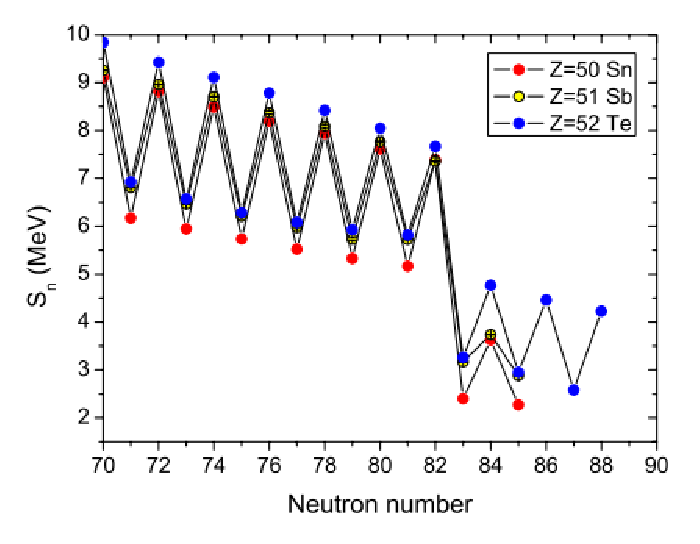
\includegraphics[width=100mm]{images/S_n.eps}
 \end{center}
  \caption{Separation energy for Sn, Sb, Te isotopes as a function of neutron number obtained from experimental data \cite{KJJ12}.}
  \label{S_n}
\end{figure}

\begin{figure}[htbp]
 \begin{center}
    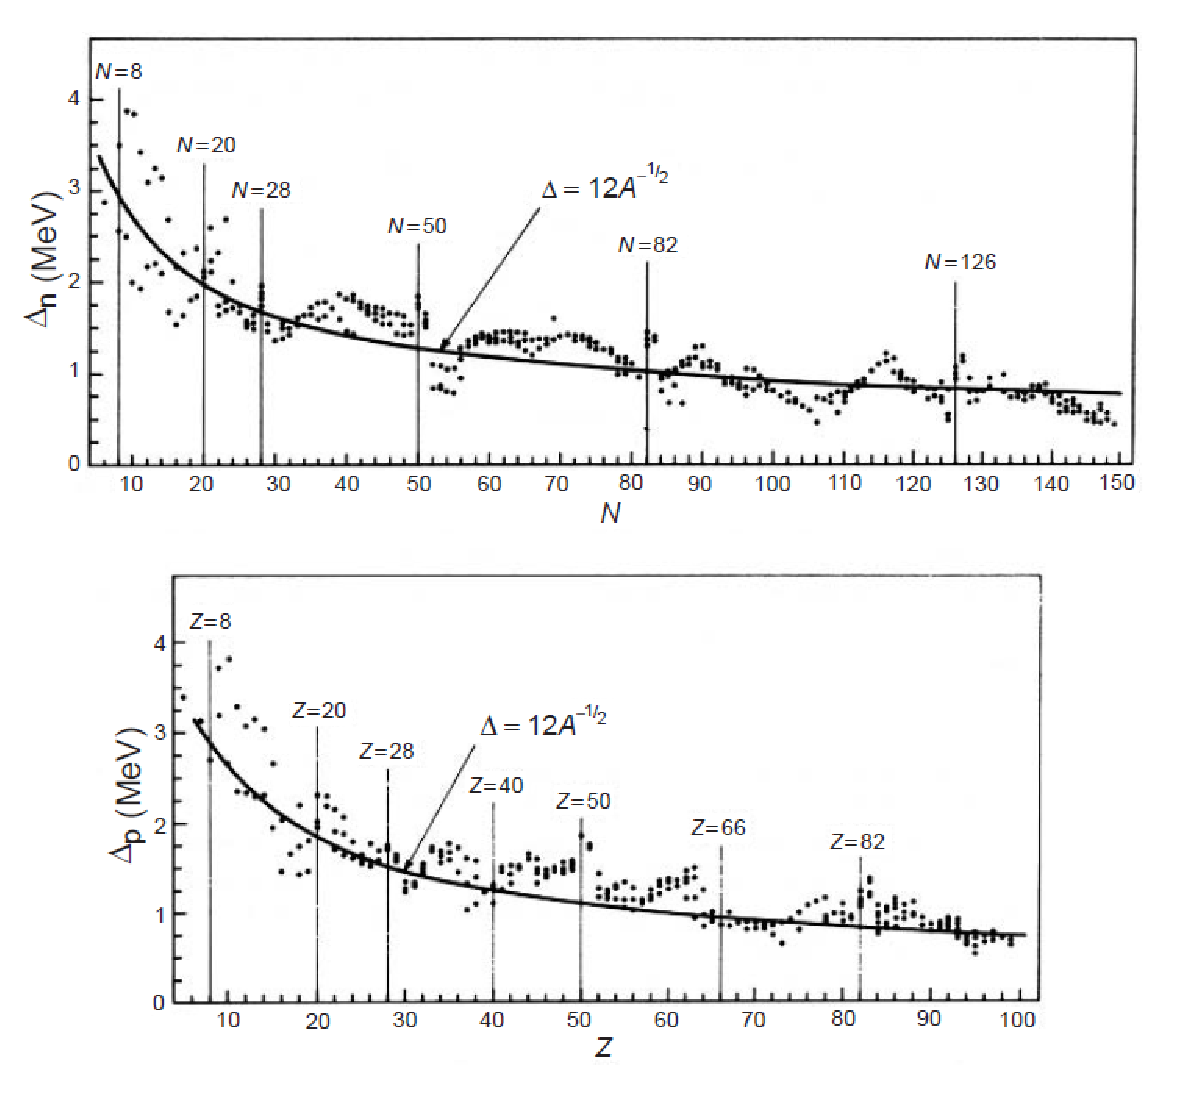
\includegraphics[width=120mm]{images/gap.eps}
 \end{center}
  \caption{The odd-even mass differences $\Delta_n$, $\Delta_p$ for neutrons and protons (Zeldes {\it et al.} {\it Mat. Fys. Skr. Dan. Vid. Selsk.}, 3, no. 5 (1967)).}
  \label{gap}
\end{figure}

Because pairing correlation is two-body interaction, a theoretical framework beyond the mean field model seems to be necessary. However, there is a tricky approximated theory, BCS theory, enable us to describe pairing correlation within mean field model. In BCS theory, the ground state is superposed by the states with different particle number. It indicates that the ground state breaks symmetry in a space, namely U(1) gauge space. With symmetry breaking, the corresponding order parameter, pairing gap $\Delta$, has finite value. Based on BCS theory, because the energy of each particle in a $J^{\pi}=0^+$ pair is $E_k=\sqrt{(\epsilon_k-\lambda)^2+\Delta^2}$, where $\epsilon_k$ is single particle energy, $\lambda$ is Fermi energy, the minimum excitation energy is $2\Delta$. In fact, pairing gap corresponds to the separation energy difference between even-even nuclei and odd mass number nuclei discussed in previous paragraph. As same as superconductivity in condensed matter physics, the superfluid nucleus is defined when $\Delta\neq0$ in ground state. Thus, the OES detected from experiment caused from pairing correlation can be well explained by BCS theory.

After BCS theory was firstly introduced by J. Bardeen, L. Cooper, and J. R. Schrieffer in 1957, it was immediately generalized to Hartree-Fock-Bogoliubov (HFB) theory. HFB theory is the naturally extension of Hartree-Fock (HF) theory by introducing Bogoliubov transformation. Under Bogoliubov transformation, the particles become to quasiparticles, and the mean field potential is extended to generalized form including pairing field. After HFB theory had been applied to nuclear physics in 1958, the structure of ground states in nuclei was examined by plenty of studies. Up to now, HFB theory is the standard mean field theory to describe nuclear structure including pairing correlation.

% Recently, nuclear density functional theory has been developed based on HFB theory. and the computational codes are well developed. The properties of ground states in even-even nuclei are well studied by HFB theory.

%BCS theory is firstly introduced by J. Bardeen, L. Cooper, and J. R. Schrieffer in 1957 \cite{} to describe . BCS theory can describe the superconducting state or superfluid state caused by cooper pairs. In nuclear physics, the  created by pairing correlation correspond to the cooper pairs. 

%  It indicates that the ground states consist of the $J^{\pi}=0^+$ pairs is more stable than other configurations. In addition, the ground states between even-even nuclei and neighborhood odd nuclei has large gaps of binding energy. In odd nuclei, the unpaired last neutron is the last single-particle level. The odd-even mass difference  To break the $J^{\pi}=0^+$ pair, we need large energy which

%Pairing correlation plays an important role near the Fermi energy.
%\begin{figure}[htbp]
% \begin{center}
%    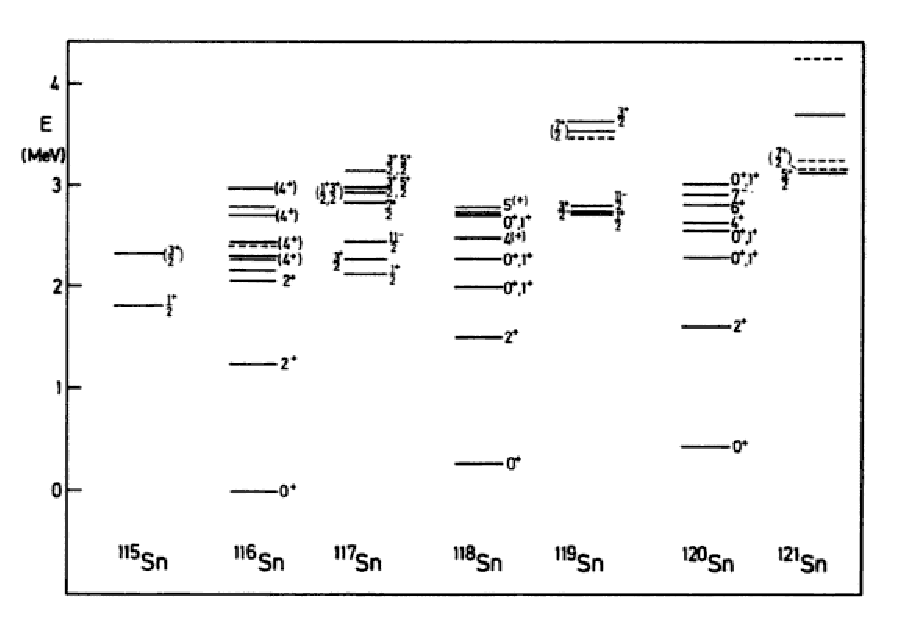
\includegraphics[width=100mm]{images/Sn_isotope.eps}
% \end{center}
%  \caption{Low-lying excited states in Sn isotopes \cite{}. The absolute values of binding energy are adjusted at 0 MeV in the ground state of ${}^{116}$Sn.}
%  \label{Sn_isotope}
%\end{figure}


\subsection{Pairing collective motion}
\label{1-1-2}
Due to the superfluid state breaks the symmetry in U(1) gauge space, we expect that there are two types of elementary modes of excitation for pairing collective motion in nuclei. Two types of elementary modes of excitation are Nambu-Goldstone (NG) mode, pairing rotation, recovering the broken symmetry in U(1) gauge space, and Higgs mode, pairing vibration, fluctuating around the energy minimum point.

\begin{figure}[htbp]
 \begin{center}
    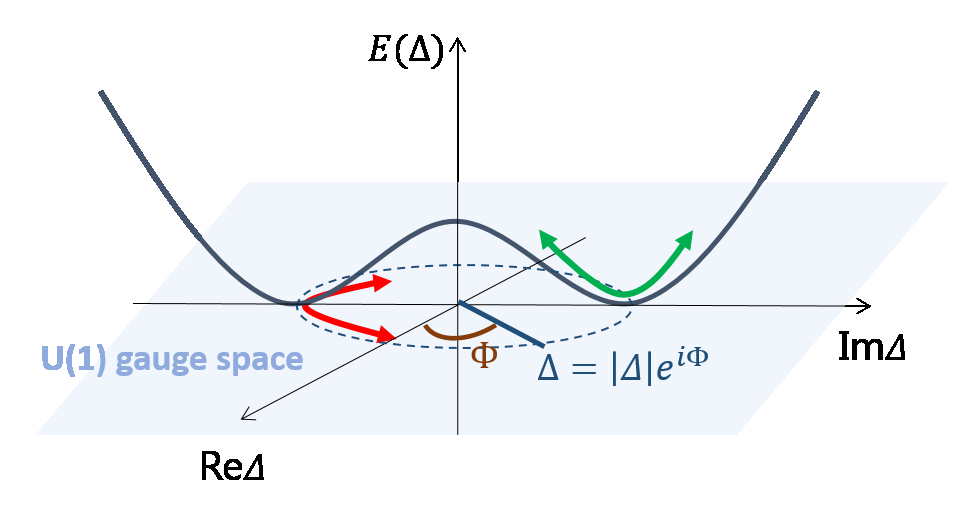
\includegraphics[width=100mm]{images/pair_coll.eps}
 \end{center}
  \caption{Schematic picture of pairing collective motion with superfluid ground state. Red  bi-direction arrow indicates pairing rotation, which rotates in $\Phi$ direction along the energy minimum circle degenerating at an absolute value of pairing gap $|\Delta|\neq 0$, in U(1) gauge space. Green bi-direction arrow indicates pairing vibration, which vibrates in $|\Delta|$ direction around one of the degenerated energy minimum points.}
  \label{Pair_coll}
\end{figure}
First, we discuss about pairing rotation. In classical picture, pairing rotation is the motion which the system rotates in the U(1) gauge space (red bi-direction arrow in Fig. \ref{pair_rot}). The motion is described by the coordinate, gauge angle $\Phi$, and the corresponding momentum, total particle number $N$. 
%It is similar to normal rotation in 3D space which described by the angles ($\theta_x, \theta_y, \theta_z$) and their conjugate angular momenta ($J_x, J_y, J_z$). 
Because the total particle number is unchanged in time evolution, the momentum $N$ is conserved quantity. In quantum picture, if we assume the ground state in a particle number $N_0$ as the ``ground state'', the ground states in $N=N_0\pm2, N_0\pm4,\cdots$ correspond to the ``excited states'' of pairing rotational mode. The excitation energy is $E_{\rm rot}^{\rm pair}=\frac{(N-N_0)^2}{2\mathcal{J}}$, where $\mathcal{J}$ is the pairing-rotational moment of inertia which characterizes the pairing rotation. In experiment, the pairing rotational band is expected to be observed in even-even isotope chain or even-even isotone chain between two magic numbers. One clear observation is found in Sn isotopes shown in Fig. \ref{pair_rot}. Except  a constant value and linear term with respect to mass number $A$, we can find the energies of ground states consist of a parabolic line - pairing rotational band. Recently, the systematic study for the pairing-rotational moment of inertia has been done in Ref. \cite{HN16}. The experimental moments of inertia obtained from two neutron(proton) separation energies have excellent correspondence with the theoretical moments of inertia obtained from NG mode in quasiparticle random phase approximation (QRPA) \cite{TV61} based on HFB mean field theory, not only for the spherical nuclei, but also for the deformed nuclei. Because the pairing-rotational moments of inertia are free from ambiguities caused from odd-even system, they are supposed to be excellent indicators of pairing correlation rather than pairing gaps.

Next, we discuss about pairing vibration. We emphasize that there are two types of pairing vibrations, one which vibrates around normal ground state ($\Delta\approx 0$), and another one which vibrates around superfluid ground state ($\Delta\neq 0$). The structures between two vibrational modes are quite different. 
%The former one is well understood because the structure of the excited $0^+$ states are $2np2nh$ configurations, detected from the energy spectra around ${}^{208}$Pb. 
Here, we only focus on the later one.
In classical picture, the later one vibrates around one of the degenerated energy minimum points. Depending on the intrinsic structure, various pairing vibrations can exist in one nucleus. 
%In general, the motion is supposed to be described by the coordinate, pairing gap $\Delta$, and its corresponding momentum\footnote{Because $\Delta$ is order parameter, it is naturally supposed to be the coordinate to describe the pairing vibration in previous studies. However, we found $\Delta$ is not proper coordinate in most of case from our study. The detail is discussed in Chapter 3 and 4.}.
In quantum picture, if we assume the ground state in a particle number $N_0$ as the ``ground state'', the excited states in $N=N_0, N_0\pm2, N_0\pm4,\cdots$ correspond to the ``excited states'' of pairing vibrational mode. The excitation energy is $E_{\rm vib}^{\rm pair}=n_{\alpha}\hbar\omega$, where $n_{\alpha}$ is the number of phonon and $\alpha$ is the label to distinguish different pairing vibrational modes. Because $2\Delta$ is the minimum energy to break one-pair, the collectivity is supposed to be strong when $E_{\rm vib}^{\rm pair}<2\Delta$. Thus, low-lying excited $0^+$ states in even-even nuclei are possible to be pairing vibrational states. Except the region around the magic number, excited $0^+$ states below $2\Delta$ exist in most of even-even nuclei. However, it is difficult to observe the signatures for pairing vibration directly from experiment. The properties of pairing vibration in nuclei are not well understood up to now.

The signatures for pairing collective motion can also be observed from the two-neutron(proton) transfer reaction \cite{BHR73}, such as $(p, t)$, $(t, p)$, and $({}^3{\rm He}, n)$. The cross sections of two particle transfer reaction strongly depend on the matrix elements of $J^{\pi}=0^+$ pair-transition operators (e.g. pair-additional transition: $\sigma( P_{ad};0_{\alpha}^+(N) \to 0_{\beta}^+(N+2))\sim |\braket{N+2,\beta|\sum_k a^{\dag}_k a^{\dag}_{\bar{k}}|N,\alpha}|^2$). From theoretical prediction, the pairing correlation is known to enhance $\sigma(g.s.\to g.s.)$ and decrease $\sigma(g.s.\to 0_{ex}^+)$ significantly, hence, $\sigma(g.s.\to 0_{ex}^+)/\sigma(g.s.\to g.s.)\ll 1$ is expected in superfluid system. One example of $(p, t)$ reactions is demonstrated in Fig. \ref{pair_rot}. As mentioned in previous paragraph, the ground states of even-even Sn isotopes consist of a pairing rotational band. In such situation, we can find intraband transition is dominant with respect to interband transition. Therefore, the cross sections of two-neutron transfer reaction is consistent with theoretical prediction. In general, the ratio $\sigma(g.s.\to 0_{ex}^+)/\sigma(g.s.\to g.s.)$ for two-neutron(proton) transfer reaction are excellent indicators to describe the collectivity of pairing dynamics.

\begin{figure}[htbp]
 \begin{center}
    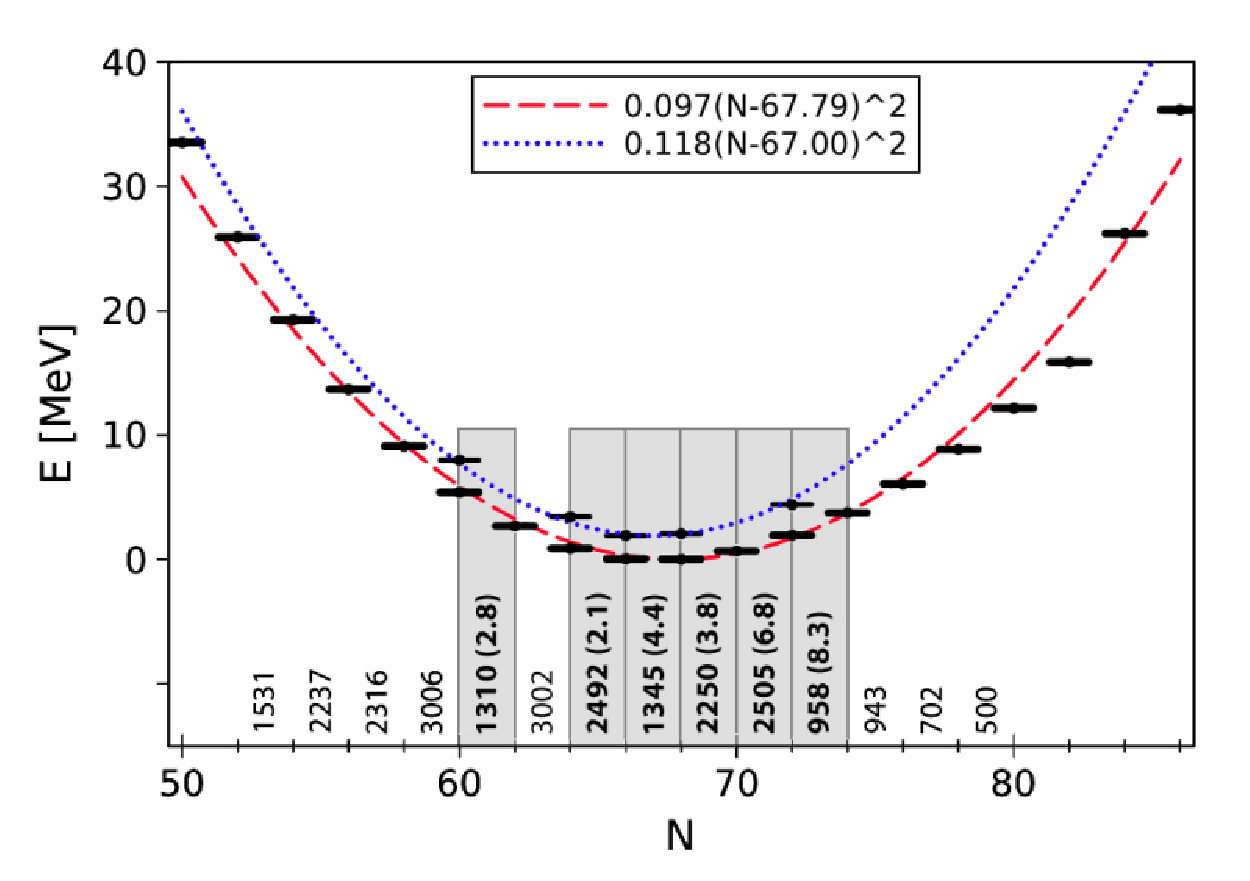
\includegraphics[width=100mm]{images/pair_rot.eps}
 \end{center}
  \caption{Experimental energies of the $J^{\pi}=0^+$ states of the Sn isotopes (ground state and pairing vibration),
populated in $(p, t)$ reactions. The heavy drawn horizontal lines
represent the values of the expression $E=-B({}_{50}^{A}{\rm Sn}_{N})+E_{exc}+
8.124A+46.33$ MeV, where $B({}_{50}^{A}{\rm Sn}_{N})$ is the binding energy
of the Sn isotopes of mass number $A$, and $E_{exc}$ is the
weighted [with $\sigma(0_i^+)$] average energy of the excited $0^+$ states
below 3 MeV. The dashed and dotted lines represent the parabolas
given in the insets, corresponding to the ground state and to
the (average) excited state-based pairing rotational bands. The
absolute values of the $g.s.\to g.s.$ integrated cross sections (in $\mu$b units) are given (perpendicular) to the abscissa, as a function
of $N$. The values in the shaded areas correspond to the experimental values, while the remaining values correspond to theoretical
predictions. For the first group (experimental), the relative
(in \%)$(p, t)$, pairing vibrational, cross sections $\sum_i\sigma(g.s.\to 0_i^+)$
normalized with respect to the ground state cross sections are in parenthesis. The detailed information are written in \cite{PF11}.}
  \label{pair_rot}
\end{figure}

\section{Motivation of this study}

\subsection{Mysterious excited $0^+$ states and pairing dynamics}
In most of nuclei, the structure of excited $0^+$ states is complicate and unclear. The reason is that not only pairing correlation but also deformations and multipole correlations influence the excited $0^+$ states significantly. The various correlations competing with each other construct plenty of mysterious excited $0^+$ states.

After the concept of pairing vibration was introduced, it encountered the problem for the large asymmetry cross sections between $(p, t)$ and $(t, p)$ reaction in actinide region observed from experiment. In low-lying energy region, the cross section of $\sigma(g.s.\to 0_{ex}^+)$ is about $15\%$ of $\sigma(g.s.\to g.s.)$ for $(p, t)$ reaction \cite{MEFSS70, MEFSS72}, while the signal of $\sigma(g.s.\to 0_{ex}^+)$ is extremely weak for $(t, p)$ reaction \cite{Cas72}. To explain such phenomena, the coexistence of both oblate shape and prolate shape in one state, and the mixing of pairing correlations between oblate and prolate shape was suggested \cite{GJV71,RK72}. Another interpretation for such phenomena is using microscopic interaction, including multipole pairing correlations and quadrupole particle-hole interactions \cite{RB76}. Although the approaches are different, they succeeded to reproduce the asymmetry cross section of two-neutron transfer reaction in actinide region.

$\beta$ vibration
Collective motion is the essential idea to explain the excited states in nuclei. The quadrupole collective motion described by the quadrupole deformation parameters $\alpha_{2\mu} (\mu=\pm2,\pm1,0)$ is known as the most typical collective motion. In the framework of quadrupole collective motion, the low-lying excited $0^+$ states can be roughly categorized into two types: quadrupole vibration emerging above two-phonon excitation in spherical nuclei, and $\beta$ vibration emerging in quadrupole deformed nuclei. The excitation energies and $B(E2)$ transition strength is well understood under harmonic approximation.

\subsection{Theoretical problem}
%As discussed in previous section, the low-lying excited $0^+$ states are not be understood in general. 
We aim to understand the mysterious excited $0^+$ states discussed in previous section based on mean field approach. In low-energy region, the pairing correlation supposed to be important as the quadrupole correlation. The most well-known and successful model is Bohr model, which was introduced to describe low-energy nuclear collective motion in quadrupole degrees of freedom with the deformation parameters $(\beta,\gamma)$ and the Euler angles $(\phi,\theta,\psi)$. However, the pairing degrees of freedom is not included in the Bohr model. As discussed in Sec. \ref{1-1-2}, the pairing vibrational degrees of freedom supposed to be a key ingredient to understand the low-lying  excited $0^+$ states.
 the pairing vibrational degrees of freedom is necessary to include in the collective model. the role of pairing correlation is hardly discussed up to now.
The degrees of freedom for pairing collective motion are supposed to be necessary including the collective model.

The study about the collective model for pairing collective motion was firstly introduced by Bes. et al. \cite{BBPK70}. They constructed phenomenological pairing collective model  by two degrees of freedom, the pair deformation parameter (pairing gap) $\Delta$ and the global gauge angle $\Phi$. After the pairing collective model was formulated, it was applied to several studies for nuclear structure \cite{GPBW85, ZPPRS99, P07}. 
In Ref. \cite{ZPPRS99}, the $B(E2)$ transition improved by introducing pairing degrees of freedom. On the other hand, the wave function of ground state from collective model looks like unusual because the pairing gap $\Delta_{vib}$ at the peak of the wave function is smaller than the pairing gap $\Delta_{eq}$ obtained from BCS equation. 

It is supposed to be important to find the collective coordinates describing the pairing collective motions from the microscopic degrees of freedom without any assumption. 

The difficult point is the requantization of the pairing collective motion. Such difficulty is not found in quadrupole collective motion.

\subsection{Our idea}

\subsection{Outline of this thesis}
In this study, we concentrate in the pairing model which only contains pairing interaction in two-body interaction to construct the theoretical framework of the requantization.


\chapter{Pairing model}

To examine the pairing dynamics influencing the structure of nuclei, we can only concentrate the nucleons near the Fermi energy. The Hamiltonian of pairing model is
\begin{align}
	H &= \sum_{l=1}^L \epsilon_l n_l - g \sum_{l,l'} S_l^+ S_{l'}^- ,
\end{align}
where
\begin{align}
	n_l &= \sum_m a^{\dag}_{lm}a_{lm} \\
        S_l^{+} &= \sum_{m>0}a_{lm}^{\dag}a_{l\overline{m}}^{\dag} ,
\quad   S_l^{-} = S_l^{+\dag} .
\label{S_+}
\end{align}
In $L$ single-particle level system, each single-particle energy $\epsilon_l$ possesses $(2\Omega_l)$-fold
degeneracy ($\Omega_l=j_l+1/2$)
and $\sum_{m>0}$ indicates the summation over $m=1/2,3/2,\cdots,$ and $\Omega_l-1/2$. $\overline{m}$ indicates the time reversal quantum number with respect to $m$. The strength of pairing correlation is represented by coupling constant $g$. We also define a seniority $\nu_l$, which is the number of unpaired particles in each level. The total number of unpaired particles is $\nu=\sum_l\nu_l$. The unpaired particles have no pairing interaction, and play a part in Pauli blocking effect.\par
In one-level system ($L=1$), the pairing dynamics is well understood. The analytic solution of the total energy is
\begin{align}
	E_{\nu}(N) = \epsilon N - \frac{1}{4}g(N-\nu)(2\Omega-N-\nu+2) .
	\label{onelevel}
\end{align}
The pairing rotational band created by the pairing correlation is completely parabolic with the moment of inertia $2/g$. Also, the excited states in a specified $N$ is only described by the quantum number $\nu$. For example, the first excited state in even particle system is $\nu=2$ state, which correspond to one $J^{\pi}=0^+$ pair broken state.\par
The profound dynamics occurs in multi-level pairing model ($L\ge 2$). The pairing rotational mode becomes complex due to the shell effect. In addition, several pairing vibrational modes emerge. The pairing vibration is not single particle motion specified by $\nu_l$, but a collective motion with the excitation of $J^{\pi}=0^+$ pairs. In this chapter, we explain the numerical exact solution and derive the TDHFB dynamics in multi-level pairing Hamiltonian.

\section{Exact solution}
The eigenvalues and eigenvectors can be solved exactly in pairing model. There are two major methods to obtain the exact solutions, diagonalization in quasispin space and Richardson equation.

\subsection{Diagonalization in quasispin space}
We introduce SU(2) quasispin operators fulfilling the follows commutation relation
\begin{equation}
  [S_l^0,S_{l'}^{+}] = \delta_{ll'}S_{l}^{+},\hspace{20pt}[S_{l}^{+},S_{l'}^{-}] = 2\delta_{ll'}S_{l}^{0}. 
  \label{SU2commu}
\end{equation}
If we set 
\begin{align}
  S_l^0 &= \frac{1}{2}(\sum_ma_{lm}^{\dag}a_{lm}-\Omega_l)
  \label{S_0}
\end{align}
and $S_l^+, S_l^-$ are the same as in (\ref{S_+}), the commutation relation (\ref{SU2commu}) is fulfilled. Using quasispin operators, the Hamiltonian can be represented by quasispin operators
\begin{align}
	H &= \sum_l \epsilon_l (2S_l^0+\Omega_l) - g \sum_{l,l'} S_l^+ S_{l'}^- .
\end{align}
Therefore, any states $\ket{\psi}$ belong to SU(2)$\otimes\cdots\otimes$SU(2) Hilbert space, and can be expanded in the basis $\ket{S_1,S_1^0;\cdots;S_l,S_l^0;\cdots}$
\begin{equation}
  \ket{\psi} = \sum_{S_1^0,\cdots\,S_l^0,\cdots}c_{S_1^0,\cdots\,S_l^0,\cdots}\ket{S_1,S_1^0;\cdots;S_l,S_l^0;\cdots} .
\end{equation}

We discuss the physical meaning of the quasispin space. Because $S_l^+$ and $S_l^-$ correspond to the creation and annihilation operators with respect to the $J^{\pi}=0^+$ pairs in each level, the quasispin space is decoupled from the space which the unpaired particles belong to. 
Also, $S_l^0$ is related to the occupation number in each level. $S_l^0=-S_l$ is the minimum value corresponding no $J^{\pi}=0^+$ pair in the level and $S_l^0=S_l$ is the maximum value corresponding full of $J^{\pi}=0^+$ pairs in the level. Because $\nu_l$ plays a part in Pauli blocking effect in the level, the absolute value of quasispin $S_l$ is
\begin{equation}
  S_l = \frac{1}{2}(\Omega_l-\nu_l).
\end{equation}

The dimension of the model space is $D=\prod_l(2S_l+1)$. However, $[H,N]=0$ indicates that the Hamiltonian is block diagonal with respect to the total particle number $N$. The model space can be reduced after we extract the combination of $\{S_l^0\}$ fulfilling
\begin{equation}
  N = \sum_l (2S_l^0+2S_l+\nu_l) .
\end{equation} 
For example, we consider the dimension of the single particle levels between the magic number 50 and 82. Under spherical symmetry, we have five single particle levels, $d_{5/2}$, $g_{7/2}$, $s_{1/2}$, $d_{3/2}$, and $h_{11/2}$. The corresponding degeneracy is $\{\Omega_l\}=\{3,4,1,2,6\}$. If we only consider the case for$\nu_l=0$, the dimension for the system is $D=840$. On the other hand, under a specified $N$, the dimensions are 105 for $N=14$ and 91 for $N=20$.

\subsection{Richardson equation}
As mentioned above, diagonalizing the Hamiltonian is simple method to obtain the exact solution.
However, diagonalization is time consuming when the model space becomes large. The calculation time is proportional to the cubes of the dimension of the model space For example, there are 16 single particle levels between the magic number 50 and 82 in deformed nuclei. Because the dimension for the system is $D=2^{16}=65536$, the calculation time in deformed system is $\sim 10^5$ times as much as the case in spherical system. \par
The alternative method to obtain the exact solution is to solve Richardson equation. The idea was introduced by R. W. Richardson \cite{Richardson1, Richardson2, Richardson3}. We divide the total energy into two parts
\begin{align}
  E &= \braket{\psi|H|\psi} \\
  &= \sum_l \epsilon_l \nu_l + \sum_{\alpha=1}^M E_{\alpha} .
\end{align}
The first term is the energy of unpaired particle, and the second term is the total energy of $J^{\pi}=0^+$ pairs. The pair-energy $E_{\alpha}$ is derived from the non-linear equations
\begin{equation}
  1 - g\sum_l \frac{\Omega_l-\nu_l}{2\epsilon_l-E_{\alpha}} + 2g\sum_{\beta(\neq\alpha)}^M \frac{1}{E_{\beta}-E_{\alpha}} = 0 .
\end{equation}
$M$ indicates the number of $J^{\pi}=0^+$ pairs in the system, and equals to the numbers of the non-linear equations. $E_{\alpha}$ can become not only real numbers, but also complex conjugate pairs when $M\ge 2$. 

\section{TDHFB dynamics}
%In realistic nuclear system with nuclear effective interaction, the necessary model space is huge. To diagonalize the effective Hamiltonian is extremely difficult task. Such study is done by shell model calculation. In alternative way, we only prepare a limited model space, which supposed to be reproduce the important parts of nuclear properties. The time-dependent mean-field theory 
To understand the classical picture of the pairing dynamics, time-dependent mean-field (TDMF) theory is useful tool. With pairing correlation, TDMF theory attributes to TDHFB theory.
The TDHFB equation can be derived from the time-dependent variational principle,
\begin{equation}
  \delta\mathcal{S}=0, \quad 
  \mathcal{S} \equiv \int \braket{\phi(t)|i\frac{\partial}{\partial t}-H|\phi(t)}dt ,
  \label{variation}
\end{equation}
where $\ket{\phi(t)}$ is the time-dependent generalized Slater determinant (coherent state) obtained from Thouless' theorem
\begin{equation}
  \ket{\phi(t)} = \mathcal{R}\exp{\left( \sum_{k<k'}Z_{kk'}(t)\beta_k^{\dag}\beta_{k'}^{\dag}
    \right)}\ket{\Phi_0} .
\end{equation}
$\beta_k^{\dag}$ is quasiparticle creation operator and $\mathcal{R}$ is normalization factor. $\ket{\Phi_0}$ is generally chosen as ground state or vacuum state. $Z_{kk'}(t)$ is time-dependent complex number determined by TDHFB equation.

\subsection{Hamilton's equation}
We derive the TDHFB equation in pairing model. First, we consider the time-dependent coherent state. Because the noticeable phenomenon is the dynamics for $J^{\pi}=0^+$ pairs in pairing model, we can describe the time-dependent coherent state in SU(2) quasispin space. Using Thouless' theorem, the time-dependent coherent state becomes
\begin{equation}
	\ket{Z(t)} = \prod_{l} \left(1+|Z_l(t)|^2\right)^{-S_l}
	\exp [Z_l(t) S_l^{+}] \ket{0} .
 \label{coherent}
\end{equation}
Here, we choose $\ket{\Phi_0}=\ket{0}$ which is vacuum (zero particle) state. In the quasispin representation, $\ket{0}=\prod_l \ket{S_l,-S_l}$. The coherent state is the extension of BCS trail wave function, which consists of the superposition of different particle number states. $Z_l$ are complex numbers. $|Z_l|=0$ corresponds to empty occupation and $|Z_l|=\infty$ corresponds to full occupation for $J^{\pi}=0^+$ pairs.\par
 With the transformation $Z_l = \tan{\frac{\theta_l}{2}}e^{-i\chi_l}$ ($0\leq\theta\leq\pi$, $0\leq\chi<2\pi$), the Lagrangian and the expectation value of Hamiltonian become
\begin{align}
	\mathcal{L}(t) =& \braket{Z(t)|i\hbar\frac{\partial}{\partial t}-H|Z(t)}
	=\sum_l j_l\dot{\chi_l} - \mathcal{H}(\chi,j) ,\\
	\mathcal{H}(\chi,j) \equiv& \braket{Z(t)|H|Z(t)} \nonumber \\
	=& \sum_l \epsilon_l\nu_l + \sum_l 2\epsilon_lj_l - g\sum_l \left( (\Omega_l-\nu_l) j_l - j_l^2 +\frac{j_l^2}{\Omega_l-\nu_l} \right) \nonumber \\
	&- 2g\sum_{l_1<l_2} \sqrt{j_{l_1}j_{l_2}(\Omega_{l_1}-\nu_{l_1}-j_{l_1})(\Omega_{l_2}-\nu_{l_2}-j_{l_2})}\cos{(\chi_{l_1}-\chi_{l_2})}   ,
	\label{Hamiltonian}
\end{align}
where $\chi_l$ are the canonical coordinates and $j_l$ are the conjugate momenta defined in
\begin{align}
  j_l\equiv \frac{\partial\mathcal{L}}{\partial\dot{\chi}_l}=S_l(1-\cos{\theta}_l) .
  \label{momenta}
\end{align}
The detailed derivations are written in Appendix \ref{derivation}. The canonical variables $(\chi,j)$ have clear physical meaning. $\chi_l$ represent a kind of gauge angle of each level, and $j_l$ correspond to the occupation number of each level
\begin{align}
  \braket{Z|n_l|Z} = \nu_l + 2j_l .
  \label{occ}
\end{align}
From (\ref{momenta}), we can find that $0\le j_l\le 2S_l$, where $j_l=0$ corresponds to empty occupation and $j_l=2S_l$ corresponds to full occupation for $J^{\pi}=0^+$ pairs.
Using canonical variables, the TDHFB equations attribute to the Hamilton's equations
\begin{equation}
	\dot{\chi_l} = \frac{\partial\mathcal{H}}{\partial j_l}, \quad
	\dot{j_l} = -\frac{\partial\mathcal{H}}{\partial \chi_l} .
\end{equation}

\subsection{Constant of motion}
\label{constant}
The number of the TDHFB degrees of freedom is same as the number of the single-particle levels. However, because the Hamiltonian depends only on the relative difference in the gauge angles, the global gauge angle 
\begin{align}
	\Phi = \frac{1}{L}\sum_l \chi_l
\end{align}
is a cyclic variable. With the definition for relative gauge angle (e.g. $\phi_l = \chi_l-\chi_1$), we can find that the conjugate momentum of $\Phi$ is the sum of $j_l$
\begin{align}
	J \equiv \frac{\partial\mathcal{L}}{\partial\dot{\Phi}} = \sum_l j_l .
\end{align}
From (\ref{occ}), $J$ is related to the total particle number
\begin{align}
	N = \nu + 2J .
\end{align}
The Hamilton's equation for $J$
\begin{align}
	\dot{J} = -\frac{\partial\mathcal{H}}{\partial \dot{\Phi}} = 0, \quad J = {\rm const}
\end{align}
indicates that the total particle number is conserved in time evolution.
The canonical variable $(\Phi,J)$ describes the pairing rotation. The pairing rotational band emerges in the particle number chain ($\cdots,N-2,N,N+2,\cdots$). The last term in (\ref{Hamiltonian}) contains the higher order terms with respect to $N$. It related to the shell effect. In single-level system, the last term in (\ref{Hamiltonian}) disappears and (\ref{Hamiltonian}) attributes to (\ref{onelevel}). The pairing rotational band is exactly parabolic. In multi-level system, the coupling constant $g$ and single-particle energy $\epsilon_l$ affects significantly to the last term in (\ref{Hamiltonian}). The parabolic structure can be broken when the shell effect is strong. 

In the analysis of TDHFB classical Hamiltonian, we can decouple the pairing rotational mode. The degrees of freedom is $L-1$ in $L$ level system. Therefore, the dynamics is integrable for $L=2$ and non-integrable for $L\le 3$ in multi-level pairing model. We discuss the integrable system and non-integrable system in Chapter \ref{integrable} and \ref{non-integrable}, respectively. 

\chapter{Requantization of TDHFB in integrable system}
\label{integrable}
As discussed in Sec. \ref{constant}, the TDHFB dynamics in two-level system is one-dimensional motion. We know that one-dimensional system must be integrable system. 
There are two new discoveries obtained from the study of the integrable system. First, the requantization method, stationary phase approximation to the path integral, can be applied straightforward to describe the collective excited $0^+$ states. We find that SPA is superior to the other requantization methods, especially for the calculation of two-particle transition strength. Second, the collective coordinates are explicit in integrable system. Using the explicit collective coordinates, we can examine the performance of the collective model which assumes the pairing gap parameter as the collective coordinate. The conclusion is the pairing gap parameter can only describe a part of collective space, and the applicability of the collective model is limited.

\section{Classical dynamics in two-level system}
\subsection{TDHFB dynamics}
To describe the one-dimensional motion, we introduce the global gauge angle $\Phi$ and the relative gauge angle $\phi$ as canonical coordinates
\begin{align}
  \Phi &\equiv \frac{\chi_1 + \chi_2}{2}, \quad\quad
  \phi\equiv \chi_2 - \chi_1.
\label{phi}
\end{align}
These ranges are $0\leq \Phi \leq 2\pi$ and $-2\pi \leq \phi \leq 2\pi$. 
Their conjugate momenta $(J,j)$ are given by
\begin{align}
	J = \frac{\partial\mathcal{L}}{\partial\dot{\Phi}} =  \sum_{l=1}^2 j_l, 
 \quad\quad
j = \frac{\partial\mathcal{L}}{\partial\dot{\phi}} = \frac{j_2 - j_1}{2}.
	\label{pi}
\end{align}
As in (\ref{occ}), $j$ corresponds to relative occupation number
\begin{align}
  j = \frac{\nu_{2}-\nu_{1}}{2} + \frac{n_{2}-n_{1}}{4}
\end{align}
The Lagrangian and Hamiltonian in terms of these canonical variables
$(\phi,j;\Phi,J)$ are given by
\begin{align}
	\mathcal{L} =& J\dot{\Phi} + j\dot{\phi} - \mathcal{H}(\phi,j;J) \label{Lagrangian2}\\
	\mathcal{H}(\phi,j;J)
	=& \sum_{l=1,2} \epsilon_l\nu_l + \sum_{l=1,2} 2\epsilon_lj_l - g\sum_{l=1,2} \left( (\Omega_l-\nu_l) j_l - j_l^2 +\frac{j_l^2}{\Omega_l-\nu_l} \right) \nonumber \\
	&- 2g\sqrt{j_1j_2(\Omega_{1}-\nu_{1}-j_{1})(\Omega_{2}-\nu_{2}-j_{2})}\cos{\phi} , 
\label{Hamiltonian2}
\end{align}
with 
\begin{align}
	j_1 = \frac{J}{2} - j, \quad\quad j_2 = \frac{J}{2} + j .
	\label{j_l}
\end{align}
The TDHFB equation can be written in a form of
the classical equations of motion:
\begin{eqnarray}
	&&\frac{d\Phi}{dt} = \frac{\partial\mathcal{H}}{\partial J} ,\quad\quad
\frac{dJ}{dt} = -\frac{\partial\mathcal{H}}{\partial \Phi} , \\
	&&\frac{d\phi}{dt} = \frac{\partial\mathcal{H}}{\partial j} ,\quad\quad
\frac{dj}{dt} = -\frac{\partial\mathcal{H}}{\partial \phi} .
\label{TDHFB_equation}
\end{eqnarray}
Because $J$ and the total energy $E$ constants of motion, the TDHFB trajectories with given $J$ and $E$ are determined
in the two-dimensional phase space $(\phi,j)$ with the condition
\begin{equation}
  \mathcal{H}(\phi(t),j(t);J) = E.
  \label{contour}
\end{equation}

\begin{figure}[tp]
 \begin{center}
  \includegraphics[width=60mm,angle=-90]{images/phase.eps}
 \end{center}
 \caption{Energy contour plot for $\Omega_1=\Omega_2=8$ and $N=16$.
	The lines indicate the TDHFB trajectories fulfilling
	the EBK quantization condition of Eq. (\ref{EBK}).
	}
 \label{fig:phase_space}
\end{figure}

We show an example of the classical trajectories in two-level system. Fig. \ref{fig:phase_space} is the contour lines fulfilling (\ref{contour}), which correspond to the classical trajectories, with $\Omega_1=\Omega_2=\Omega=8$, $\nu=0$, and $N=2\Omega=16$ with various coupling constant $g$. The dimensionless coupling constant $x$ is defined as $x=2g\Omega/(\epsilon_2-\epsilon_1)$ (See Appendix \ref{two-level}). The phase transition from normal state to superfluid state occurs at $x=1$ in closed shell ($N=2\Omega$). At $x<1$ corresponding the left panel in Fig. \ref{fig:phase_space}, the trajectory of ground state is $j=-4$ independent from $\phi$. It is consistent with the fully occupied lower level $n_1=N$ and the empty upper level $n_2=0$. For the dynamical states, the trajectories are open with gentle slopes. At $x>1$ corresponding the middle and right panels in Fig. \ref{fig:phase_space}, the trajectory of ground state becomes a point at $\phi=0$, $j=j_0$ $(-4<j_0<4)$. With superfluid ground state, the dynamical states have two types, closed trajectory and open trajectory. The closed trajectory appears around $(\phi,j)=(0,j_0)$ at low-energy region. On the other hand, the open trajectory with steep slope appears at high-energy region relatively. The stronger pairing correlation, the higher excitation energy of the transition point from closed trajectory to open trajectory. The structure of the excited states between closed trajectory and open trajectory is quite different. They influence the matrix element of two-particle transfer reaction significantly. We will discuss the feature of the excited states in the following sections.

\subsection{Adiabatic TDHFB (ATDHFB) dynamics}
\label{ATDHFB}
In general collective motion, the frequency in the collective motion is much smaller than the frequency in single particle motion ($\hbar\omega\ll\epsilon_m-\epsilon_i$). The slow velocity of the collective motion enable us to expand the collective Hamiltonian up to second order with respect to the collective momentum (adiabatic approximation). We discuss the behavior of TDHFB dynamics in adiabatic approximation.\par
From (\ref{Hamiltonian2}), we find that the classical Hamiltonian is even function with respect to $\phi$. With time reversal $t\to-t$, (\ref{TDHFB_equation}) is invariant under $j\to j, \phi\to -\phi$, which indicates that $j$ is time even and $\phi$ is time odd. Thus, we switch the coordinate and momentum 
\begin{equation}
	(\phi,j)\to(j,-\phi) ,
	\label{switch}
\end{equation}
to make the coordinate time even. The classical Hamiltonian under adiabatic approximation becomes
\begin{align}
  \mathcal{H}(j,\phi) &\approx V(j) + \frac{1}{2}B^{-1}(j)\phi^2,
  \label{ATDHFB_Hamiltonian}
\end{align}
where 
\begin{align}
	V(j) = \mathcal{H}(\phi=0,j) 
	=& \sum_{l=1,2} \epsilon_l\nu_l + \sum_{l=1,2} 2\epsilon_lj_l - g\sum_{l=1,2} \left( (\Omega_l-\nu_l) j_l - j_l^2 +\frac{j_l^2}{\Omega_l-\nu_l} \right) \nonumber \\
	&- 2g\sqrt{j_1j_2(\Omega_{1}-\nu_{1}-j_{1})(\Omega_{2}-\nu_{2}-j_{2})} \\
	B^{-1}(j) = \left. \frac{\partial^2\mathcal{H}}{\partial\phi^2} \right|_{\phi=0}
	=& 2g\sqrt{j_1j_2(\Omega_{1}-\nu_{1}-j_{1})(\Omega_{2}-\nu_{2}-j_{2})} .
	\label{mass_two_level}
\end{align}
It is obvious that $V(j)$ is potential and $B(j)$ is mass parameter. Because the closed trajectories appear around the energy minimum point $(\phi,j)=(0,j_0)$, we can expect that adiabatic approximation performs excellent for closed trajectories.
\begin{figure}[htbp]
 \begin{center}
  \includegraphics[width=60mm,angle=-90]{images/phase_compare.eps}
 \end{center}
 \caption{Energy contour plot in the same system as Fig. \ref{fig:phase_space}. Black solid lines correspond to TDHFB trajectories and gray dashed lines correspond to ATDHFB trajectories. 
	}
 \label{fig:phase_compare}
\end{figure}

We compare the difference of the classical trajectories between TDHFB and ATDHFB. Fig. \ref{fig:phase_compare} shows both TDHFB and ATDHFB trajectories in the same system as in Fig. \ref{fig:phase_space}. For weak pairing correlation ($x<1$), both results are similar, especially at the low-energy region. For strong pairing correlation ($x>1$), both results are almost identical for closed trajectories. The opened trajectories are also well reproduced near the closed trajectories. The deviation becomes large at the high-energy region. In conclusion, ATDHFB is excellent approximation at low-energy region, regardless of the type of the trajectories.


\section{Requantization methods}
To obtain the excited states, quantization of the TDHFB trajectory, namely, requantization is necessary procedure. The straightforward requantization method is canonical quantization, which is commonly applied into nuclear collective model. We expected canonical quantization gives reasonable result and we applied it at first. However, we find that canonical quantization has serious problem to describe the pairing dynamics. To solve or avoid the problem, alternative requantization methods, Fourier decomposition and stationary phase approximation to the path integral, are also introduced. In this section, we explain each requantization method in detail, respectively.

\subsection{Stationary phase approximation to the path integral}
At first, we introduce the idea of stationary phase approximation to the path integral (SPA). Starting an arbitrary state $\ket{\psi(0)}$ at time $t=0$,
the time-dependent full quantum state can be written in the path integral form
\begin{align}
\ket{\psi(t)}
	=& e^{-iHt} \ket{\psi(0)} \nonumber \\
	=& \int d\mu(Z'') \ket{Z''} \int d\mu(Z') \int_{Z(0)=Z'}^{Z(t)=Z''} \mathcal{D}\mu[Z(\tau)]
	e^{i\mathcal{S}[Z(\tau)]} \psi(Z') ,
\label{path_integral_expression}
\end{align}
where $\psi(Z)\equiv \braket{Z|\psi(0)}$ and
the invariant measure $d\mu(Z)$ is defined by 
the unity condition,
\begin{equation}
  \int d\mu(Z) \ket{Z}\bra{Z} = 1 .
  \label{unity}
\end{equation}
In Eq. (\ref{path_integral_expression}),
$\mathcal{S}[Z(\tau)]$ is the action (\ref{variation}) along a given path $Z(\tau)$
with the initial coherent state $\ket{Z(0)}=\ket{Z'}$ and
the final state $\ket{Z(t)}=\ket{Z''}$,
then, the integration $\int \mathcal {D}\mu[Z(\tau)]$
is performed over all possible paths $\ket{Z(\tau)}$ between them.
Among all trajectories in the path integral,
the lowest stationary-phase approximation $\delta S_{\rm cl}=0$ selects
the TDHFB (classical) trajectories\footnote{
In this formulation, the stationary-phase approximation agrees with
the TDHF(B) trajectories, while that to the auxiliary-field path
integral of Refs. \cite{Neg82,L80}
leads to the TDH(B) without the Fock potentials.
}.
\begin{equation}
	\ket{\psi(t)} \approx \int d\mu(Z') \ket{Z'_{\rm cl}(t)}
	e^{i\mathcal{S}_{\rm cl}(Z'_{\rm cl}(t),Z')} \psi(Z') ,
	\label{SPA}
\end{equation}
where the TDHFB trajectory starting from $\ket{Z'}$
ends at $\ket{Z'_{\rm cl}(t)}$ at time $t$.
The action $\mathcal{S}_{\rm cl}(Z_f,Z_i)$ is calculated along this
classical trajectory
connecting $Z_i=Z'_{\rm cl}(0)=Z'$ and $Z_f=Z'_{\rm cl}(t)$.
\begin{align}
	\mathcal{S}_{\rm cl}(Z'_{\rm cl}(t),Z') &\equiv \int_{0}^{t}
\braket{Z_{\rm cl}(t)|
	i\frac{\partial}{\partial t} - H
	|Z_{\rm cl}(t)} dt \nonumber \\
	&= \mathcal{T}[Z_{\rm cl}] - \mathcal{H}(Z',Z'^*) t 
	,
	\label{S_cl}
\end{align}
with the action integral $\mathcal{T}[Z_{\rm cl}]$
\begin{align}
\mathcal{T}[Z_{\rm cl}] &\equiv
\int_{0}^{t} \braket{Z_{\rm cl}(t)| i\frac{\partial}{\partial t}
	|Z_{\rm cl}(t)} dt  .
\end{align}
In the last equation of Eq. (\ref{S_cl}),
we used the fact that the TDHFB trajectory conserves the energy,
$\mathcal{H}(Z_{\rm cl}(t),Z_{\rm cl}^*(t))= \mathcal{H}(Z',Z'^*)$.
%We assume that only classical (TDHFB) trajectory contributes to the time dependent wave function

The energy eigenstates correspond to stationary states,
$\braket{Z|\psi(t)} \propto \braket{Z|\psi(0)}=\psi(Z)$,
which can be constructed by superposing the coherent states along
a periodic TDHFB trajectory $Z_{\rm cl}^{(k)}$ as \cite{KS80,K81,SM88}
\begin{equation}
	\ket{\psi_k} = \oint d\mu(Z_{\rm cl}^{(k)}) \ket{Z_{\rm cl}^{(k)}}
	e^{i\mathcal{T}[Z_{\rm cl}^{(k)}]} .
\end{equation}
The single-valuedness of the wave function leads to
the quantization condition ($k$: integer)
\begin{align}
	\mathcal{T}_\circ[Z_{\rm cl}^{(k)}]=&
	\oint \braket{Z_{\rm cl}(t)| i\frac{\partial}{\partial t}
	|Z_{\rm cl}(t)} dt  \nonumber \\
	=& 2k\pi .
	\label{EBK}
\end{align}
The state evolves in time as $\ket{\psi_k(t)}=\ket{\psi_k}e^{-iE_k t}$,
with the energy of the $k$-th periodic trajectory,
$E_k=\mathcal{H}(Z_{\rm cl}^{(k)},Z_{\rm cl}^{(k)*})$.

Finding TDHFB trajectories satisfying the quantization condition
(\ref{EBK}) is an extremely difficult task in general.
It is better founded and more practical
if the classical system is completely integrable.
In integrable systems, $M$ complex variables $Z(t)$ can be transformed into
the action-angle variables;
\begin{align}
	Z(t) &= \{Z_l(t);l=1,\cdots,M \} \nonumber \\
	&\rightarrow
	\{E; v_1,\cdots,v_{M-1}; \theta_1(t),\cdots,\theta_M(t)\} ,
\end{align}
where the variables $E$ and $v$ define an invariant torus,
while $\theta(t)$ parameterize the coordinates on the torus.
The integration path of Eq. (\ref{EBK}) is now taken as topologically
independent closed path on the torus,
namely the EBK quantization condition.
There are $M$ independent closed paths and $M$ quantum numbers,
$k=(k_1,\cdots,k_M)$, to specify the stationary energy eigenstate.
These are associated with $M$ invariant variables,
$\{E_k;v_1^{(k)},\cdots,v_{M-1}^{(k)}\}$.
Using the invariant measure
\begin{align}
%  d\mu(Z) = \rho(Z)dEdv_1\cdots dv_{M-1}d\theta_1\cdots d\theta_M,
  d\mu(Z) = \rho(E,v,\theta) dEdv_1\cdots dv_{M-1}d\theta_1\cdots d\theta_M,
\end{align}
the $k$-th semiclassical wave function can be calculated as
\begin{align}
  \ket{\psi_k} \propto \oint d\theta_1\cdots \oint d\theta_M &\ 
	\rho(E_k,v^{(k)},\theta)
	\ket{E_k,v^{(k)},\theta} \nonumber \\
	&\times e^{i\mathcal{T}[E_k,v^{(k)},\theta]} .
  \label{semi_wave_func}
\end{align}
Here, we omit the integration with respect to the invariant variables,
$E$ and $v$.

We apply the SPA approach to the two-level pairing model.
The invariant measure in SU(2)$\otimes$SU(2) is 
\begin{align}
%	d\mu(Z) &= \prod_{l=1,2} \frac{S_l+1}{\pi}(1+|Z_l|^2)^{-2}d{\rm Re}Z_ld{\rm Im}Z_l \\
%  &= \prod_l \frac{S_l+1}{4\pi}\sin{\theta_l}d\theta_ld\phi_l \\
%  &= \frac{S_1+1}{4\pi}\frac{S_2+1}{4\pi}\frac{1}{S_1S_2}d\Phi d\Pi d\phi d\pi .
d\mu(Z) &= \prod_l \frac{\Omega_l+1}{\pi}(1+|Z_l|^2)^{-2}d{\rm Re}Z_ld{\rm Im}Z_l \\
  &= \prod_l \frac{\Omega_l+1}{4\pi}d\cos{\theta_l}d\chi_l \\
	&= \left(\prod_{l=1,2} \frac{1+\Omega_l^{-1}}{2\pi}\right)
             d\Phi dJ d\phi dj .
\end{align}
In the last equation, we transform the canonical coordinates
by Eqs. (\ref{phi}) and (\ref{pi}).
Since the particle number $J=N/2$ and the total energy $E$ are invariant,
the two-level pairing model is integrable.
Thus, we can construct the semiclassical wave function using
Eq. (\ref{semi_wave_func}).
From (\ref{Lagrangian2}), the action integral is given by
\begin{align}
	\mathcal{T}_k(\Phi,\phi;J)
	&= J\Phi + \int^t_0
	j(t') \frac{d\phi}{dt'} dt' \nonumber \\
	&\equiv \mathcal{T}_{N,E_k}(\Phi,t) ,
\end{align}
where the integration is performed on the $k$-th
closed trajectory of Eq. (\ref{EBK}), and
the variables $(\phi,j)$ are transformed into $(t,E)$.
%where $\pi(t)$ can be solved from the right side of (\ref{TDHFB_equation}). (i.e. 2D Runge-Kutta method) \par
The semiclassical wave function fulfilling the EBK quantization condition
becomes
\begin{align}
	\ket{\psi_k^J} &\propto \oint d\Phi \oint dt
	e^{i\mathcal{T}_{J,E_k}(\Phi, t)}
	\ket{\Phi,t}_{N,E_k} \label{semi_wave_func0} \\
  &\propto \sum_{m=0}^{J}C_m^{(E_k,J)}\ket{S_1,-S_1+m;S_2,-S_2+(J-m)} ,
	\label{semi_wave_func1}
\end{align}
with $S_l=(\Omega_l-\nu_l)/2$ and the coefficients
\begin{align}
  C_m^{(E_k,J)} =& \binom{J}{m}\int_0^T dt \nonumber \\
 &\times \exp{\left( i\int^t j(t') \dot{\phi}(t') dt'-i(J/2-m)\phi(t) \right)} \nonumber \\ 
 &\times A(j_1,S_1,m)A(j_2,S_2,J-m) ,\\
  A(j,S,m) &= \left(\frac{j}{2S}\right)^{m/2}\left(\frac{2S-j}{2S}\right)^{S-m/2}\sqrt{\frac{(2S)!m!}{(2S-m)!}}, \hspace{5mm} \nonumber
\end{align}
where $T$ is the period of the closed trajectory.
The TDHFB-requantized wave functions (\ref{semi_wave_func1}) are
eigenstates of the total particle number.
This is due to the integration over the global gauge angle $\Phi$,
which makes the particle number projection not only for the ground state
but also for excited states.
See Appendix for detailed derivation of Eq.~(\ref{semi_wave_func1}). 

Since we obtain the microscopic wave function of every eigenstate,
the expectation values and the transition matrix elements for any operator
can be calculated in a straightforward manner.
In Sec.~\ref{sec:results}, we show those of the pair-addition operator
$S^+$ which characterize properties of the pair condensates.

Before ending this section, let us note the periodic conditions
of the coordinates and the quantization condition.
Since the two original variables, $(\chi_1,\chi_2)$,
are independent periodic variables of the period $2\pi$,
in addition to the trivial periodicity of $2\pi$ for $\Phi$ and of $4\pi$
for $\phi$,
we have periodic conditions for
$(\Phi,\phi)\rightarrow (\Phi\pm \pi,\phi\pm 2\pi)$ and
$(\Phi,\phi)\rightarrow (\Phi\pm \pi,\phi\mp 2\pi)$.
The former (latter) corresponds to $\chi_2\pm 2\pi$ ($\chi_1\pm 2\pi$)
with $\chi_1$ ($\chi_2$) being fixed.
For open TDHFB trajectory (e.g., Fig.~\ref{fig:phase_space}),
the quantization condition becomes
\begin{align}
 \mathcal{T}_{J,E_k}(\Phi\pm\pi,\phi\pm 2\pi;J) &= \mathcal{T}_{J,E_k}(\Phi,\phi;J) + 2m\pi \nonumber \\
	 \Leftrightarrow \quad\quad \pm J \pi + \int_{-\pi}^\pi j d\phi
	&= 2m\pi .
\end{align}
This leads to the following:
\begin{equation}
	\int_{-\pi}^\pi j d\phi = 
	\begin{cases}
		2k\pi & \mbox{ for } J=2n ,\\
		(2k+1)\pi & \mbox{ for } J=2n+1 ,
	\end{cases}
	\label{EBK_2}
\end{equation}
where $m$, $k$ and $n>0$ are integer numbers.


\subsection{Canonical quantization}
\label{sec:canonical}
In the pairing collective model, the canonical quantization
was adopted in previous studies \cite{BBPK70,delta1,delta3}.
Assuming magnitude and phase of the pairing gap as collective coordinates,
a collective Hamiltonian was constructed in the second order in momenta.
Then, the Hamiltonian was quantized by the canonical quantization
with Pauli's prescription.
In this section, we apply similar quantization method to
the TDHFB Hamiltonian (\ref{TDHFB_Hamiltonian_3}).
The main difference is that the collective canonical variables are
not assumed in the present case, but are obtained from the TDHFB dynamics
itself.\par
It is not straightforward to apply Pauli's prescription
to the present case, 
because the TDHFB Hamiltonian (\ref{Hamiltonian2})
is not limited to the second order in momenta.
In the present study, 
we adopt a simple symmetrized ordering, as
\begin{align}
	\mathcal{H}(\hat{\phi},\hat{j};\hat{J})
	=& \sum_{l=1,2} \epsilon_l\nu_l + \sum_{l=1,2} 2\epsilon_lj_l - g\sum_{l=1,2} \left( (\Omega_l-\nu_l) j_l - j_l^2 +\frac{j_l^2}{\Omega_l-\nu_l} \right) \nonumber \\
	&- g \left\{ \sqrt{j_1j_2(\Omega_{1}-\nu_{1}-j_{1})(\Omega_{2}-\nu_{2}-j_{2})}\cos{\hat{\phi}} \right. \nonumber \\
	&\left. + \cos{\hat{\phi}}\sqrt{j_1j_2(\Omega_{1}-\nu_{1}-j_{1})(\Omega_{2}-\nu_{2}-j_{2})} \right\} .
\label{canonical_quantized_H}
\end{align}
To fulfill the canonical quantization condition
\begin{align}
 [\hat{\Phi},\hat{J}]=i, \quad\quad [\hat{\phi},\hat{j}]=i ,
\end{align}
as in (\ref{j_l}), $j_l$ contain $J$ and $j$ which
are replaced by
\begin{equation}
	\hat{J} = -i\frac{\partial}{\partial\Phi},\quad\quad
	\hat{j} = -i\frac{\partial}{\partial\phi} .
\end{equation}
Since $\Phi$ is a cyclic variable, 
we write the collective wave function $\Psi(\Phi,\phi)$ as eigenstates
of the number of $J^{\pi}=0^+$ pairs $J$ in a separable form
\begin{equation}
  \Psi_k^{(J)}(\Phi,\phi) = 
	\frac{1}{\sqrt{2\pi}}e^{iJ\Phi}\psi_k^{(J)}(\phi) .
\end{equation}
Then, the problem is reduced to the one-dimensional Schr\"{o}dinger
equation for the motion in the relative angle $\phi$.
%pairing vibrational mode can be obtained by solving
the Schr\"{o}dinger equation is
\begin{equation}
	H\left( \phi,-i\frac{d}{d\phi};J \right)
	\psi_k^{(J)}(\phi) = E_k^{(J)}\psi_k^{(J)}(\phi) .
	\label{Schroedinger_eq}
\end{equation}

The wave function should have a periodic property with respect to
the variable $\phi$;
$\psi_k(\phi)=\psi_k(\phi+4\pi)$.
For the adopted simple ordering of Eq. (\ref{canonical_quantized_H}),
it is convenient to use the eigenstates of $\hat{j}$ as the basis
to diagonalize the Hamiltonian.
They are
\begin{equation}
%  \hat{\pi}\chi_\nu(\phi) = \nu \chi_\nu(\phi) \\
	\chi_j(\phi) = \frac{1}{\sqrt{4\pi}} e^{i\phi j} ,
	\quad\quad\mbox{with $j$: integer or half integer} .
\end{equation}
Since the Hamiltonian (\ref{canonical_quantized_H}) contains only
terms linearly proportional to $e^{\pm i\phi}$,
the basis states $\chi_j$ with half-integer difference in $j$
are not coupled with each other.
Thus, the eigenstates of Eq. (\ref{Schroedinger_eq}) can be expanded as
\begin{equation}
	\psi_k^{(J)}(\phi) = 
	\sum_{j=j_{\rm min},j_{\rm min}+1,\cdots}^{j_{\rm max}}
	c_{k,j}^{(J)} \chi_j^{(J)}(\phi) .
	\label{CQ_eigenstate}
\end{equation}
According to the relation $j=(j_2-j_1)/2$ in Eq. (\ref{pi}),
we adopt the (half-)integer values of $j$ for $J=2n$ ($J=2n+1$)
with integer $n$.
This is consistent with the quantization condition (\ref{EBK_2}).
The coupling term with different $j$
in Eq. (\ref{canonical_quantized_H}) vanishes
for $j_l=0$ and $j_l=\Omega_l-\nu_l$,
which restricts values of $j$ in a finite range of
$j_{\rm min}\leq j \leq j_{\rm max}$.

In order to estimate the two-particle transfer matrix elements,
we construct the corresponding operators as follows.
The classical form of matrix elements are obtained as
\begin{align}
  S^+(\Phi,J;\phi,j) &= \braket{Z|\hat{S}^+|Z} \nonumber \\
 &= \frac{1}{2}
\left( \sqrt{j_1(\Omega_1-\nu_1-j_1)}e^{-i\phi/2}+\sqrt{j_2(\Omega_2-\nu_2-j_2)}e^{i\phi/2} \right) e^{i\Phi}
	\label{Sp_mean_value} \\
  S^-(\Phi,J;\phi,j) &= \braket{Z|\hat{S}^-|Z} \nonumber \\
 &= \frac{1}{2}
\left( \sqrt{j_1(\Omega_1-\nu_1-j_1)}e^{i\phi/2}+\sqrt{j_2(\Omega_2-\nu_2-j_2)}e^{-i\phi/2} \right) e^{-i\Phi} .
	\label{Sm_mean_value}
\end{align}
%For simplicity, we ignore the part of off-diagonal element (e.g. $\braket{Z'|\hat{S}_+|Z}$). 
%To requantize the two-particle transition operators, 
Again, we adopt a simple symmetrized ordering for the quantization:
\begin{align}
%  &S_+(\Phi,\Pi;\phi,\pi) \to S_+(\hat{\Phi},\hat{\Pi};\hat{\phi},\hat{\pi}) \nonumber \\
  S^\pm (\hat{\Phi},\hat{J};\hat{\phi},\hat{j})
	=& \frac{1}{4}\left( \sqrt{j_1(\Omega_1-\nu_1-j_1)}e^{\mp i\hat{\phi}/2}
+\sqrt{j_2(\Omega_2-\nu_2-j_2)}e^{\pm i\hat{\phi}/2} \right) e^{\pm i\hat{\Phi}} \nonumber \\ 
&+ \frac{1}{4}e^{\pm i\hat{\Phi}}\left( 
e^{\mp i\hat{\phi}/2}\sqrt{j_1(\Omega_1-\nu_1-j_1)}
+e^{\pm i\hat{\phi}/2}\sqrt{j_2(\Omega_2-\nu_2-j_2)} \right) .
\end{align}
The exponential factors $e^{\pm i\Phi}$ change
the total particle number $N\rightarrow N\pm 2$ ($J\rightarrow J\pm 1$),
while $e^{\pm i\phi/2}$ change the relative numbers,
$j_2-j_1 \rightarrow j_2-j_1 \pm 1$.
%For example, the pair-additional transition strength in requantized form is
Using these operators,
the pair-addition transition strengths are calculated as
\begin{align}
B(P_{\rm ad};k\rightarrow k') &=
|\braket{J',k'|S^+(\hat{\Phi},\hat{J};\hat{\phi},\hat{j})|J,k}|^2
	\nonumber \\
&= \left| \frac{1}{2\pi} \int_{0}^{2\pi}d\Phi \int_{-2\pi}^{2\pi}d\phi 
	\psi^{(J')*}_{k'}(\phi) e^{-iJ'\Phi}
	S^+(\hat{\Phi},\hat{J};\hat{\phi},\hat{j})
	\psi^{(J)}_{k}(\phi)e^{iJ\Phi} \right|^2,
\end{align}
which automatically vanishes for $J'\neq J+1$.


\subsection{Fourier decomposition}
\label{sec:Fourier}

The requantization and calculation of the matrix elements can be also
performed using the time-dependent solutions of the TDHFB.
It was proposed and applied to the two-level pairing model \cite{CDS84},
which we recapitulate in this section.

The TDHFB provides a time-dependent solution $Z(t)$ starting from
a given initial state $Z(0)$.
The energy eigenvalues and the corresponding closed trajectories
are determined from the EBK quantization condition (\ref{EBK}).
The pair transfer matrix elements are evaluated as the Fourier components
of the time-dependent mean values $S^\pm(t)=S^\pm(Z(t))$,
Eqs. (\ref{Sp_mean_value}) and (\ref{Sm_mean_value}).
%In the ground state, the motion in the global gauge angle $\Phi$
%is independent from the $\phi$ motion.
Since the global gauge angle $\Phi$ is a cyclic variable,
the motion in the relative gauge angle $\phi$ is independent from $\Phi$.
Thus, we calculate the time evolution of $\phi(t)$, and
find the period of the $k$-th closed trajectory $T$
satisfying Eq. (\ref{EBK}).
Then, the Fourier component,
\begin{equation}
	\tilde{S}^\pm(E_k; \omega) = \frac{1}{T}\int_0^T dt
	e^{i\omega t} S^\pm(t) ,
\label{Fourier_decomposition}
\end{equation}
corresponds to the pair transfer matrix element from the state $k$ to $k'$
when $\omega=2\pi (k'-k)/T$.
The pair-addition transition strengths are calculated as
\begin{equation}
	B(P_{\rm ad};k\rightarrow k') 
	= \left|\tilde{S}^+\left(E_k;\frac{2\pi}{T}\Delta k \right) \right|^2 ,
\end{equation}
with $\Delta k=k'-k$.
In this approach, the transition between the ground states of
neighboring nuclei ($N\rightarrow N+2$) corresponds to
the stationary component ($k=0$ and $\Delta k=0$),
namely the expectation value in the BCS approximation.

The derivation  of Eq. (\ref{Fourier_decomposition})
is based on the wave packet in the
classical limit \cite{LL65}.
The TDHFB state is assumed to be a superposition of eigenstates $\ket{\phi_k^N}$
in a narrow range of energy $E_{k_0}-\Delta E<E_k<E_{k_0}+\Delta E$,
\begin{equation}
	\ket{Z(t)} = \sum_N \sum_k c_k^N \ket{\phi_k^N} e^{-iE_k t} ,
	\label{superposition}
\end{equation}
where the eigenenergies are evenly spaced and
the coefficients $c_k^N$ slowly vary with respect to $k$ and $N$.
The expectation value of $S^\pm$ is
\begin{equation}
	S^\pm(t) = \sum_{N} \sum_{k,k'} c_{k'}^{N+2*} c_k^N 
	\braket{\phi_{k'}^{N+2}|S^\pm|\phi_k^N} e^{i(E_{k'}-E_k)t} .
\end{equation}
The matrix element $\braket{\phi_{k'}^{N+2}|S^\pm|\phi_k^N}$
quickly disappears as $|k'-k|$ increases, while it stays almost constant
for the small change of $k$ and $N$ with $|k'-k|$ being fixed.
Thus, we may approximate $c_{k'}^{N+2}\approx c_k^N$,
$E_{k'}-E_k\approx \omega_0 \Delta k$, and
that $\braket{\phi_{k'}^{N+2}|S^\pm|\phi_k^N}\approx
\braket{\phi_{k_0+\Delta k}^{N+2}|S^\pm|\phi_{k_0}^N}$ 
\begin{align}
	S^\pm(t) &\approx \sum_{N} \sum_{k} \left|c_k^N\right|^2
	\sum_{\Delta k}
	\braket{\phi_{k_0+\Delta k}^{N+2}|S^\pm|\phi_{k_0}^N}
	e^{i\omega_0 \Delta k t}  \nonumber \\
	&= \sum_{\Delta k}
	\braket{\phi_{k_0+\Delta k}^{N+2}|S^\pm|\phi_{k_0}^N}
	e^{i\omega_0 \Delta k t}  ,
\end{align}
where $k_0$ is a representative index value of the superposition in 
Eq. (\ref{superposition}).
From this classical wave packet approximation,
we obtain Eq. (\ref{Fourier_decomposition}).
It is not trivial to justify the approximation for small values of $\Omega$
and for transitions around the ground state.

\section{Result}
In this section, we study the seniority-zero states ($\nu_1=\nu_2=0$) in
the two-level system with equal degeneracy, $\Omega_1=\Omega_2=\Omega$.
Since all the properties are scaled with the ratio, $g/\Delta\epsilon$,
where $\Delta\epsilon$ is the level spacing
$\Delta\epsilon=\epsilon_2-\epsilon_1$,
we use the dimensionless parameter $x$ defined in Appendix (\ref{x}) to control the strength of the pairing correlation.

We apply the requantization methods in Sec.~\ref{sec:requantization}.
In the following, the stationary-phase approximation to the path
integral in Sec.~\ref{sec:SPA} is denoted as ``SPA'',
the Fourier decomposition method (Sec.~\ref{sec:Fourier}) as ``FD'',
and the canonical quantization with periodic boundary condition 
(Sec.~\ref{sec:canonical}) as ``CQ''.
Note that the SPA and the FD produce the same eigenenergies which
are based on the EBK quantization rule.


\subsection{Large-$\Omega$ cases}

\begin{figure}[t]
 \begin{center}
(a)	 \includegraphics[height=0.6\textwidth,angle=-90]{images/N50ex_energy_wo_adiabatic.eps}
\\
(b)	 \includegraphics[height=0.6\textwidth,angle=-90]{images/N100ex_energy_wo_adiabatic.eps}
 \end{center}
 \caption{Excitation energies of $\ket{0_2^+}$, $\ket{0_3^+}$ and
$\ket{0_4^+}$ for $\Omega=50$ systems with (a) $N=50$ and (b) $N=100$
	as functions of the dimensionless parameter $x$ of Eq. (\ref{x}).
}
 \label{fig:N50energy}
\end{figure}


In the limit of $\Omega\rightarrow\infty$,
we expect that the classical approximation becomes exact.
Here, we adopt $\Omega=50$ with $N=100$ (closed-shell configuration)
and $N=50$ (mid-shell configuration).

Calculated excitation energies are shown in Fig.~\ref{fig:N50energy}.
The results of SPA/FD and CQ are compared with the exact values.
At the weak pairing limit of $x\rightarrow 0$,
the excitation energies are multiples of $2\Delta\epsilon$, 
which correspond to pure $2n$-particle-$2n$-hole excitations.
Both the weak and the strong pairing limits
are nicely reproduced by all the calculations,
while the CQ method produces excitation energies slightly lower than the
exact values in an intermediate region around $x=1$.
It is somewhat surprising to see that the deviation is larger for
the case of the mid-shell configuration ($N=50$) than the closed shell
($N=100$).

The deviation in the CQ method is mainly due to the zero-point energy
in the ground state.
Since we solve the collective Schr\"odinger equation (\ref{Schroedinger_eq})
with the quantized Hamiltonian of Eq. (\ref{canonical_quantized_H}),
the zero-point energy $\Delta E>0$ is inevitable in the CQ method.
The $\Delta E$ is associated with the degree of localization of
the wave function.
Thus, the magnitude of $\Delta E$ for ``bound'' states are different
from that for ``unbound'' states.
See Fig.~\ref{fig:phase_space}.
In the strong pairing limit, the potential minimum is deep enough to bound
both ground and excited states.
Conversely, all the states are unbound in the weak limit.
In both limits, $\Delta E$ for ground and excited states are similar,
and they are canceled for the excitation energy.
However, near $x=1$, the ground state is bound,
while the excited states are unbound.
In this case, $\Delta E$ is larger in the ground state than in the
excited states, which makes the excitation energy smaller.
This also explains the difference between the mid-shell and closed-shell
configurations.
In the closed shell, all the states are unbound for $x<1$,
while, in the mid-shell,
there is a region in $x<1$ where the ground state is bound but
the excited state is unbound.

The obtained wave functions in the SPA and the CQ can be decomposed in the
$2n$-particle-$2n$-hole components in Fig.~\ref{fig:N50_occ}.
In the SPA, it is done as Eq. (\ref{semi_wave_func1}) and
the normalized squared coefficients $|C_m^{(E_k,J)}|^2$ are plotted
in Fig.~\ref{fig:N50_occ}.
For the CQ, $|c_{k,j}^{(N)}|^2$ in Eq. (\ref{CQ_eigenstate}) are shown.
Here, $m$ and $j$ are related to each other, $2j=J-2m$.
They show excellent agreement with the exact results, not only for the
ground state but for excited states.
We find the SPA is even more precise than the CQ.
\begin{figure}[t]
 \begin{minipage}{1\hsize}
 \begin{center}
  \includegraphics[height=0.45\textwidth,angle=-90]{images/N50Xeq0p5occ_wo_adiabatic.eps}
  \includegraphics[height=0.45\textwidth,angle=-90]{images/N100Xeq0p5occ_wo_adiabatic.eps}
  \includegraphics[height=0.45\textwidth,angle=-90]{images/N50Xeq2occ_wo_adiabatic.eps}
  \includegraphics[height=0.45\textwidth,angle=-90]{images/N100Xeq2occ_wo_adiabatic.eps}
 \end{center}
 \end{minipage}
 \caption{
Occupation probability in excited $0^+$ states
as a function of $j$ for $\Omega=50$ systems
with (a) $N=50$ and (b) $N=100$.
The upper and lower panels display the results for $x=0.5$ and $x=2$,
respectively. 
The three vertical bars at each $j$ from the left to the right represent
the squared components of the wave functions
from exact, SPA, and CQ calculations, respectively.
The left end of the horizontal axis at $j=j_{\rm min}$
corresponds to a component with $(n_1,n_2)=(N,0)$.
The next at $j=j_{\rm min}+1$ corresponds to the one with
$(n_1,n_2)=(N-2,2)$, and so on.
}
 \label{fig:N50_occ}
\end{figure}

Next, let us discuss the transition matrix elements.
In this paper, we discuss only $k=0$ (ground state) and $k=1$
(1st excited $\nu=0$ state).
The FD calculation is based on the time evolution of the expectation 
value $S^+(t)$ with fixed $(J,\Phi)$ in Eq. (\ref{Fourier_decomposition}).
For $(N,k)\rightarrow (N+2,k')$ transitions,
we basically adopt the trajectories for the initial state, namely,
the one with $J=N/2$ satisfying the $k$-th EBK quantization condition.
The $k\rightarrow k$ ($\Delta k = 0$)  transitions
correspond to the intraband transitions of the
pair-rotational band, when the state is deformed in the
gauge space (pair deformation).
For the ground-state band ($k=0$),
this is nothing but the expectation value at the BCS wave function,
with the constant value of $S^+$.
Since the constant $S^+$ provides only $\Delta k=0$ intraband transitions,
for the interband transition of $(N,k=0)\rightarrow (N+2,k=1)$
transitions, the trajectory satisfying the EBK condition of $k=1$ is used to
perform the Fourier decomposition (\ref{Fourier_decomposition})
of $\omega=2\pi/T$.

\begin{figure}[t]
 \begin{minipage}{0.3\hsize}
 \begin{center}
  \includegraphics[width=70mm,angle=-90]{images/N50Pad_CQ.eps}
 \end{center}
 \captionsetup{labelformat=empty,labelsep=none}
 \end{minipage}
 \begin{minipage}{0.3\hsize}
 \begin{center}
  \includegraphics[width=70mm,angle=-90]{images/N50Pad_FD.eps}
 \end{center}
 \captionsetup{labelformat=empty,labelsep=none}
 \end{minipage}
 \begin{minipage}{0.3\hsize}
 \begin{center}
  \includegraphics[width=70mm,angle=-90]{images/N50Pad_SPA.eps}
 \end{center}
 \captionsetup{labelformat=empty,labelsep=none}
 \end{minipage}
 \caption{The strength of pair additional transition
$B(P_{\rm ad};k\rightarrow k')$ for $\Omega=50$ systems
from $N=48$ to 50.
Left panels: results of the CQ method; Middle panels: FD; Right panels: SPA.
Dashed lines represent exact calculation.
Upper panels show the intraband transitions of
$\ket{0_1^+}\to\ket{0_1^+}$ and $\ket{0_2^+}\to\ket{0_2^+}$,
while lower panels show the interband transition of
$\ket{0_1^+}\to\ket{0_2^+}$ and $\ket{0_2^+}\to\ket{0_1^+}$.
}
 \label{fig:N50Pad}
\end{figure}

\begin{figure}[t]
 \begin{minipage}{0.3\hsize}
 \begin{center}
  \includegraphics[width=70mm,angle=-90]{images/N100Pad_CQ.eps}
 \end{center}
 \captionsetup{labelformat=empty,labelsep=none}
 \end{minipage}
 \begin{minipage}{0.3\hsize}
 \begin{center}
  \includegraphics[width=70mm,angle=-90]{images/N100Pad_FD.eps}
 \end{center}
 \captionsetup{labelformat=empty,labelsep=none}
 \end{minipage}
 \begin{minipage}{0.3\hsize}
 \begin{center}
  \includegraphics[width=70mm,angle=-90]{images/N100Pad_SPA.eps}
 \end{center}
 \captionsetup{labelformat=empty,labelsep=none}
 \end{minipage}
 \caption{
The same as Fig.~\ref{fig:N50Pad} but for $N=98\rightarrow 100$.}
 \label{fig:N100Pad}
\end{figure}

The calculated pair-addition strengths $B(P_{\rm ad})$ are shown in
Fig.~\ref{fig:N50Pad} for $N=48\rightarrow 50$,
and in Fig.~\ref{fig:N100Pad} for $N=98\rightarrow 100$.
Near the closed-shell configuration ($N=98\rightarrow 100$),
the pair-addition strengths for the intraband transitions ($\Delta k=0$)
drastically increase around $x=1$.
This reflects a character change from the pair vibration ($x\lesssim 1$)
to the pair rotation ($x\gtrsim 1$).
The $B(P_{\rm ad}; k\rightarrow k)$ in the pair-rotational transitions
are about 20 times larger than those in the vibrational transitions.
The interband $B(P_{\rm ad}; 0\rightarrow 1)$ are similar to
the $B(P_{\rm ad}; 0\rightarrow 0)$ in the vibrational region
($x\lesssim 1$), because they both change the number of pair-phonon quanta
by one unit.
In contrast, $B(P_{\rm ad}; 1\rightarrow 0)$, which change the phonon
quanta by three, are almost zero.
In the pair-rotational region ($x \gg 1$),
$B(P_{\rm ad}; 1\rightarrow 0)$ and $B(P_{\rm ad}; 0\rightarrow 1)$
are roughly identical. This is because both $B(P_{\rm ad}; 1\rightarrow 0)$ 
and $B(P_{\rm ad}; 0\rightarrow 1)$ correspond to one-phonon excitation
in ``deformed'' cases ($x \gg 1$).

In the mid-shell region ($N=48\rightarrow 50$),
the intraband $B(P_{\rm ad}; k\rightarrow k)$ are smoothly increase as
$x$ increases.
Their values are larger than the interband strengths by about one (two) order
of magnitude at $x\sim 0$ ($x\sim 2.5$),
indicating the pair-rotational character.
The interband $B(P_{\rm ad}; 0\rightarrow 1)$ show a gradual decrease
as a function of $x$, while
$B(P_{\rm ad}; 1\rightarrow 0)$ are negligibly small,
even at $x\gg 1$.
This presents a prominent difference from the closed-shell case.

All the features of the pair-transfer strengths
are nicely reproduced in the SPA method,
for both the closed- and mid-shell configurations.
The CQ method qualitatively agrees with the exact calculation.
For instance, the order-of-magnitude difference between intraband
and interband transitions.
However, the precision of the CQ method is not so good,
especially around $x=1$.
The FD method properly describes the main features
in the superfluid phase, while it fails for the normal phase
($x\lesssim 1$). 
In the mid-shell configuration, the ground state is always
in the superfluid phase at $x>0$,
while the $k=1$ excited state corresponds to
the open (closed) trajectory at $0<x\lesssim 1$ ($x\gtrsim 1$).
For the open trajectory, the FD produces wrong values.
However, somewhat surprisingly,
the SPA, which uses these open trajectories for the construction
of wave functions,
reproduces main features of the exact results.


%%%%%%%%%%%%%%%%%%%%%%%%%%%%%%%%%%%%%%%%5
\subsection{Small-$\Omega$ cases}
\label{SmallOmg}

Next, we discuss systems with smaller degeneracy $\Omega=8$.
Again, we study systems near the closed-shell and the mid-shell configurations.

\begin{figure}[t]
 \begin{center}
  \includegraphics[height=0.6\textwidth,angle=-90]{images/N8ex_energy_wo_adiabatic.eps}
 \end{center}
 \caption{Excitation energies of $\ket{0_2^+}$, $\ket{0_3^+}$ and
$\ket{0_4^+}$ for $\Omega=N=8$ systems as functions of $x$.
}
 \label{fig:N8energy}
\end{figure}

\begin{figure}[htbp]
 \begin{minipage}{1\hsize}
 \begin{center}
   \includegraphics[height=0.45\textwidth,angle=-90]{images/N8Xeq0p5occ_wo_adiabatic.eps}
   \includegraphics[height=0.45\textwidth,angle=-90]{images/N8Xeq2occ_wo_adiabatic.eps}
 \end{center}
 \end{minipage}
 \caption{
Occupation probability in excited $0^+$ states
as a function of $j$ for $\Omega=N=8$ systems.
The panels (a) and (b) display the results for $x=0.5$ and $x=2$,
respectively. 
See also the caption of Fig.~\ref{fig:N50_occ}.
}
 \label{fig:N8_occ}
\end{figure}


\subsubsection{Mid-shell configuration}

The calculated excitation energies are shown in Fig.~\ref{fig:N8energy}
for the $N=8$ case.
The SPA/FD reproduces the exact calculation in the entire region of $x$,
not only for the lowest but also for higher excited states.
The CQ reproduces the exact result in a weak pairing region ($x\lesssim 1$),
while it underestimates the excitation energies at $x\gtrsim 1$.
Analogous to the case of $\Omega=50$,
this is mainly due to effect of the zero-point energy $\Delta E$.
The ground-state energy in the CQ calculation 
is bound at $x\gtrsim 1$.
However, because of the weak collectivity with $N=8$,
the first excited state stays unbound even at the maximum $x$ in 
Fig.~\ref{fig:N8energy}.
Therefore, the energy shift $\Delta E>0$ is larger in the ground state,
which makes the excitation energy smaller.

The wave functions are plotted in Fig.~\ref{fig:N8_occ}. 
At the weak pairing case of $x=0.5$,
both the SPA and the CQ reproduce the exact result.
At $x=2$, the squared coefficients of the ground state has an
asymmetric shape peaked at the
lowest $j$, which suggests that the state is not deeply bound in the
potential.
It is in contrast to the symmetric shape in Fig.~\ref{fig:N50_occ}.
The wave functions obtained by the CQ method has noticeable deviation
from the exact results.
On the other hand, the SPA wave functions are almost identical to the
exact ones.

The pair-addition transition strengths from $N=6$ to $N=8$ are
shown in Fig.~\ref{fig:N8Pad}.
The intraband $k\rightarrow k$ transitions increase and 
the interband $k=0\rightarrow 1$ transitions decrease as
functions of $x$.
Their relative difference becomes
more than one order of magnitude at $x\gtrsim 2$.
Thus, even at relatively small $\Omega$ and $N$,
the intraband transitions in the pair rotation is qualitatively different
from the interband transitions.

We find the excellent agreement between the SPA and the exact calculations.
The first excited state corresponds to the open trajectory which
turns out to almost perfectly reproduce the exact wave function.
In contrast, this open trajectory produces results far from the exact
one in the FD method.
It produces almost vanishing the intraband
$B(P_{\rm ad}; 1\rightarrow 1)$.
The $B(P_{\rm ad}; 0\rightarrow 0)$ shows a qualitative agreement for
its behavior, but is significantly underestimated.
The CQ method also underestimates the intraband transitions.

For the mid-shell configurations, the SPA is dominantly superior to the
CQ and the FD methods.

\begin{figure}[t]
 \begin{minipage}{0.3\hsize}
 \begin{center}
  \includegraphics[width=70mm,angle=-90]{images/N8Pad_CQ.eps}
 \end{center}
 \captionsetup{labelformat=empty,labelsep=none}
 \end{minipage}
 \begin{minipage}{0.3\hsize}
 \begin{center}
  \includegraphics[width=70mm,angle=-90]{images/N8Pad_FD.eps}
 \end{center}
 \captionsetup{labelformat=empty,labelsep=none}
 \end{minipage}
 \begin{minipage}{0.3\hsize}
 \begin{center}
  \includegraphics[width=70mm,angle=-90]{images/N8Pad_SPA.eps}
 \end{center}
 \captionsetup{labelformat=empty,labelsep=none}
 \end{minipage}
	\caption{The same as Fig.~\ref{fig:N50Pad} but for $N=6\rightarrow 8$
	with $\Omega=8$.
}
 \label{fig:N8Pad}
\end{figure}

\begin{figure}[htb]
 \begin{center}
  \includegraphics[height=0.6\textwidth,,angle=-90]{images/N16ex_energy_wo_adiabatic.eps}
 \end{center}
	\caption{The same as Fig.~\ref{fig:N8energy} but for
	$N=2\Omega=16$.
}
 \label{fig:N16energy}
\end{figure}

\begin{figure}[thb]
 \begin{minipage}{1\hsize}
 \begin{center}
   \includegraphics[height=0.45\textwidth,angle=-90]{images/N16Xeq0p5occ_wo_adiabatic.eps}
   \includegraphics[height=0.45\textwidth,angle=-90]{images/N16Xeq2occ_wo_adiabatic.eps}
 \end{center}
 \end{minipage}
	\caption{The same as Fig.~\ref{fig:N8_occ} but for
	$N=2\Omega=16$.
}
 \label{fig:N16_occ}
\end{figure}

\subsubsection{Closed-shell configuration}


In the closed shell with $N=16$,
the minimum-energy trajectory changes at $x=1$ from
$j=-4$ (normal phase) to
the BCS minimum $j>-4$ and $\phi=0$ (superfluid phase).
At the transitional point ($x=1$), the harmonic approximation is
known to collapse, namely to produce zero excitation energy.
In Fig.~\ref{fig:N16energy},
this collapsing is avoided in all the calculations (SPA/FD and CQ).
The behaviors of the lowest excitation agree with the exact calculations,
while the CQ method substantially underestimates those for higher states.
This is again due to the difference in the zero-point energy in
the ground and the excited states.
In the CQ calculation, the first excited state is bound at $x\gtrsim 2$,
but the second excited state is unbound for $x\lesssim 3.2$.

Near the transition point from the open to closed trajectories,
the wave functions calculated with the SPA and CQ methods somewhat differ
from the exact ones.
In Fig.~\ref{fig:N16_occ}, the wave functions at $x=0.5$ and 2 are presented.
They agree with exact calculation at $x=0.5$.
In contrast, we find some deviations for the first excited state ($k=1$)
at $x=2$.
This is because the $k=1$ trajectory corresponding to the first excited state
changes its character from open to closed at $x\approx 1.8$.
Therefore, the first excited wave function is difficult to reproduce in
the SPA, although the wave functions for
the ground and higher excited states show reasonable agreement.
The similar disagreement is observed for the ground state near $x=1$.

\begin{figure}[t]
 \begin{minipage}{0.3\hsize}
 \begin{center}
 \includegraphics[width=70mm,angle=-90]{images/N16Pad_CQ.eps}
 \end{center}
 \captionsetup{labelformat=empty,labelsep=none}
 \end{minipage}
 \begin{minipage}{0.3\hsize}
 \begin{center}
 \includegraphics[width=70mm,angle=-90]{images/N16Pad_FD.eps}
 \end{center}
 \captionsetup{labelformat=empty,labelsep=none}
 \end{minipage}
 \begin{minipage}{0.3\hsize}
 \begin{center}
 \includegraphics[width=70mm,angle=-90]{images/N16Pad_SPA.eps}
 \end{center}
 \captionsetup{labelformat=empty,labelsep=none}
 \end{minipage}
	\caption{The same as Fig.~\ref{fig:N50Pad} but for $N=14\rightarrow 16$
	with $\Omega=8$.
}
 \label{fig:N16Pad}
\end{figure}

Singular behaviors near the transition points can be also observed in
the pair-addition transition strengths ($N=14\rightarrow 16$) shown
in Fig.~\ref{fig:N16Pad}. 
At $x=1$, the intraband $B(P_{\rm ad}; 0\rightarrow 0)$ shows a kink
in the SPA,
and $B(P_{\rm ad}; 1\rightarrow 1)$ shows another kink at $x\approx 1.8$.
These exactly correspond to the transition points from open to closed
trajectories.
Nevertheless, the overall behaviors are well reproduced and
the values at the weak and strong pairing limit are reasonably reproduced
in the SPA.
The CQ calculation also shows smoothed kink-like behaviors near the
transition points.
However, it underestimates the intraband $B(P_{\rm ad}; k\rightarrow k)$.
The FD method does not have a kink for $B(P_{\rm ad}; 0\rightarrow 0)$,
because $S^+(t)$ is calculated for an $N=14$ system.
Both intraband and interband transitions in the FD calculations
reasonably agree with the exact results at $x\gtrsim 1.8$.
The $k=1$ state is not properly reproduced at $x\lesssim 1.8$
with the open trajectory.

For the closed-shell configurations,
the SPA and the FD methods provide reasonable description for the
pair-transfer transition strengths.


\section{Collective model treatment} 
The collective model has been proposed
and utilized for the nuclear pairing dynamics
\cite{BBPK70,delta1,delta3}.
For those studies, the pairing gap parameter (or equivalent quantities)
is assumed to be the collective coordinates.
This is analogous to the five-dimensional (5D) collective (Bohr) model,
in which the collective coordinates are assumed to be the
quadrupole deformation parameters, $\alpha_{2\mu}$.
The 5D collective model has been 
extensively applied to analysis on numerous experimental data.
On the contrary, there have been very few applications of
the pairing collective model
in comparison with experimental data.
In this section, we examine the validity of
the collective treatment of the pairing.

Although the global gauge angle $\Phi$ is arbitrary,
the deformation parameter $\alpha\equiv \braket{ \hat{S}^- }$
in the gauge space is
usually taken as a real value ($\Phi=0$).
%In the superfluid phase, 
The energy minimization with a fixed value of real $\alpha$ always
leads to $\phi=0$.
\begin{align}
\alpha(j,J) = \braket{Z_0|\hat{S}^-|Z_0}
	= \sqrt{j_1(\Omega_1-\nu_1-j_1)} +\sqrt{j_2(\Omega_2-\nu_2-j_2)}.
 \label{Delta_BCS}
\end{align}
The parameter $\alpha$ is equivalent to the pairing gap $\Delta$,
since the relation, $\Delta=G\alpha$,
guarantees one-to-one correspondence between $\alpha$ and $\Delta$. In Sec.~\ref{sec:canonical}, we treat $\phi$ as a collective coordinate
and $j$ as its conjugate momentum.
The collective model treatment is based on the opposite choice,
$j$ as a coordinate and $\phi$ as a momentum, as discussed in Sec. \ref{ATDHFB}.

\begin{figure}[tb]
 \begin{center}
(a) \includegraphics[height=0.44\textwidth,angle=-90]{images/N8p_E.eps}
(b) \includegraphics[height=0.44\textwidth,angle=-90]{images/N16p_E.eps}
 \end{center}
 \caption{Energy surfaces as functions of $j$,
 Eq. (\ref{TDHFB_Hamiltonian_3}) with $\phi=0$,
 for $x=0.5$, $2$, and $3.2$.
 Dashed line is the pairing deformation parameter $\alpha$
 of Eq.~(\ref{Delta_BCS}) as a function of $j$.
 (a) mid-shell ($\Omega=N=8$) and (b) closed-shell ($2\Omega=N=16$).
}
 \label{fig:p_Delta}
\end{figure}

The problem is that
there is no one-to-one correspondence between $j$ and $\alpha$.
If we examine the derivative of (\ref{Delta_BCS})
\begin{align}
\frac{\partial\alpha}{\partial j} = \frac{-(\Omega_1-\nu_1)/2+j_1}{\sqrt{j_1(\Omega_1-\nu_1-j_1)}} + \frac{(\Omega_2-\nu_2)/2-j_2}{\sqrt{j_2(\Omega_2-\nu_2-j_2)}} ,
 \label{dalpha}
\end{align}
we can find (\ref{dalpha}) is $+\infty$ for $j_{min}$ and $-\infty$ for $j_{max}$ in any two-level system. It indicates $\frac{\partial\alpha}{\partial j} =0$ exists at $j=j_0$ ($j_{min}<j_0<j_{max}$). For equal degeneracy case ($\Omega_1-\nu_1=\Omega_2-\nu_2$), $j_0=0$. 
The relation between $j$ and $\alpha$ 
are shown by dashed lines in Fig.~\ref{fig:p_Delta} 
for $\Omega=8$ mid-shell (a) and closed-shell (b) configurations discussed in Sec. \ref{SmallOmg}.
The deformation parameter $\alpha$ is largest at $j=0$ (equal filling in both levels),
and smallest at the end points of $j$.
The constrained minimization with respect to $\alpha$ cannot 
produce the states corresponding to $j>0$.
Apparently, we cannot map the entire region of $j$ to $\alpha$.

The collective model treatment
requires the collective wave functions to be well localized
in the $j<0$ region.
The potential energy, $E(j)=\mathcal{H}(\phi=0,j;J=N/2)$ of
Eq. (\ref{TDHFB_Hamiltonian_3}), is also shown in
Fig.~\ref{fig:p_Delta}.
The restriction becomes more serious for the stronger pairing cases.
For instance, the potential with $x=3.2$ in Fig.~\ref{fig:p_Delta}(a)
has only about 1 MeV depth at the minimum point, relative to the value
at the boundary point ($j=0$) corresponding to
the maximum value of $\alpha$ ($\Delta$).

To simulate the result of the collective model, we requantize the ATDHFB Hamiltonian in (\ref{ATDHFB_Hamiltonian})-(\ref{mass_two_level}) by $\hat{\phi}=i\partial/\partial j$, with
the ordering given by Pauli's prescription
\begin{align}
	H \left( j,i\frac{\partial}{\partial j} \right) 
= V(j) - \frac{1}{2}\frac{1}{\sqrt{B(j)}}\frac{\partial}{\partial j}\frac{1}{\sqrt{B(j)}}\frac{\partial}{\partial j}.
\end{align}
The range of the coordinate $j$ is restricted to $j_{\rm min}\leq j \leq 0$
with the vanishing boundary condition $\psi(j_{\rm min})=\psi(0)=0$.
Figure~\ref{fig:Delta_E} shows two examples of the relationship 
between excitation energies and the potential energy surface.
In the panel (a), we show the case of large $\Omega$
($\Omega=50$, $N=50$, and $x=2.4$),
in which
the excited $0^+$ states are bound up to second excitation.
From the collective model, the energies of the ground and the first excited states
are well described, while the deviation becomes larger for
higher excited states.
For very large degeneracy, the pocket of energy surface is deep, 
hence the low-lying excited states may be described by $\alpha$. 
However, in the small-$\Omega$ case ($\Omega=8$, $N=16$, and $x=2.4$)
of the panel (b), no excited states are bound by the potential
as a function of $\alpha$.
None of the excited $0^+$ states
are properly described in the collective model.
This shallow potential is a consequence of the improper
choice of the collective coordinate $\alpha$
which represents only the $j<0$ region.
Therefore, the collective model treatment assuming
$\alpha$ ($\Delta$) as the collective coordinate
is not applicable to small-$\Omega$ and strong-pairing cases.

\begin{figure}[tb]
% \begin{minipage}{0.45\hsize}
 \begin{center}
(a) \includegraphics[height=0.4\textwidth,angle=-90]{images/N50Xeq2p4gap_E.eps}
% \end{center}
% \end{minipage}
% \begin{minipage}{0.45\hsize}
% \begin{center}
(b) \includegraphics[height=0.4\textwidth,angle=-90]{images/N16Xeq2p4gap_E.eps}
 \end{center}
%\end{minipage}
\caption{Potential energy surface as functions of $\alpha$ with $x=2.4$;
(a) $\Omega=N=50$,
(b) $2\Omega=N=16$.
Horizontal lines 
indicate energy spectra. Black lines are obtained
from the potential energy surface, and green lines are 
obtained with the CQ method
(Sec.~\ref{sec:canonical}).
%Left panels: $\Omega=50$, $N=50$ system;
% Right panels: $\Omega=8$, $N=16$ system.
}
 \label{fig:Delta_E}
\end{figure}


\chapter{Requantization of TDHFB in non-integrable system}
\label{non-integrable}

\section{Theoretical framework of ASCC+SPA in non-integrable system}

\section{Result}

\chapter{Discussion}

\chapter{Conclusion}

\appendix


\chapter{Detailed derivation of the action in pairing model}
\label{derivation}
To obtain the TDHFB dynamics in pairing model, We need to derive the action $\mathcal{S}$ in explicit form. We give the detailed derivation in this chapter.

\section{Matrix elements of the spin-coherent state}
\label{formula1}
The time-dependent coherent state classified into the spin-coherent state is employed in (\ref{coherent}). We derive the necessary formula for the spin-coherent state in this subsection. \par
First, we consider the single-level case.
With the commutation relation in (\ref{SU2commu}), the SU(2) quasispin operators fulfill the following relations
\begin{align}
  \hat{S}^{\pm}\ket{S,S^0} &= \sqrt{(S\mp S^0)(S\pm S^0+1)} \ket{S,S^0\pm 1}
  \label{S_pm} \\
  \hat{S}^0\ket{S,S^0} &= S^0\ket{S,S^0} .
  \label{S_0}
\end{align}
Using above relations, the coherent state can be expanded as 
\begin{align}
  \ket{Z} &= (1+|Z|^2)^{-S}e^{Z \hat{S}^+}\ket{S,S^0=-S} \nonumber \\
  &= (1+|Z|^2)^{-S}\sum_{n=0}^{2S}\sqrt{\frac{(2S)!}{n!(2S-n)!}}Z^n\ket{S,-S+n} .
\end{align}
We can find the normalization condition is fulfilled
\begin{align}
  \braket{Z|Z} &= (1+|Z|^2)^{-2S}\sum_{n=0}^{2S}\frac{(2S)!}{n!(2S-n)!}|Z|^{2n} \nonumber \\
  &= (1+|Z|^2)^{-2S}\sum_{n=0}^{2S} {}_{2S}\mathrm{C}_n(|Z|^2)^n \nonumber \\
  &= (1+|Z|^2)^{-2S}\times(1+|Z|^2)^{2S} \nonumber \\
  &= 1 .
\end{align}
The overlap is
\begin{align}
  \braket{\eta|Z} &= \frac{(1+\eta^*Z)^{2S}}{(1+|\eta|^2)^S(1+|Z|^2)^S} .
\end{align}

We also calculate the expectation values of the operators. For $\hat{S}^0$,
\begin{align}
  \hat{S}^0e^{Z \hat{S}^+}\ket{S,S^0=-S} &= \sum_{n=0}^{2S}(-S+n)\sqrt{\frac{(2S)!}{n!(2S-n)!}}Z^n\ket{S,-S+n} ,
\end{align}
hence,
\begin{align}
  \braket{Z|\hat{S}^0|Z} &= (1+|Z|^2)^{-2S}\sum_{n=0}^{2S}(-S+n)\frac{(2S)!}{n!(2S-n)!}|Z|^{2n} \nonumber \\
  &= -S + 2S\left( 1-\frac{1}{1+|Z|^2} \right) \nonumber \\
  &= S\left( 1-\frac{2}{1+|Z|^2} \right) .
  \label{S0}
\end{align}
From the first line to the second line, we used the differentiation for the both sides of
\begin{align}
  (1+|Z|^2)^{2S} &= \sum_{n=0}^{2S} {}_{2S}\mathrm{C}_n(|Z|^2)^n
\end{align}
with respect to $|Z|^2$. With (\ref{S0}), the expectation values of occupation number is
\begin{align}
  \braket{Z|\hat{n}|Z} &= \braket{Z|2\hat{S}^0+\Omega|Z} \nonumber \\
	&= 2S\left( 1-\frac{2}{1+|Z|^2} \right) + \Omega .
\end{align}
The expectation values for $\hat{S}^+$ and $\hat{S}^-$ are the complex conjugate pair. For $\hat{S}^+$,
\begin{align}
  \hat{S}^+e^{Z \hat{S}^+}\ket{S,S^0=-S} &= \sum_{n=0}^{2S}\sqrt{(2S-n)(n+1)}\sqrt{\frac{(2S)!}{n!(2S-n)!}}Z^n\ket{S,-S+n+1}.
\end{align}
hence, 
\begin{align}
  \braket{Z|\hat{S}^+|Z} &= (1+|Z|^2)^{-2S}\sum_{n=0}^{2S}Z^n\sqrt{(2S-n)(n+1)}\sqrt{\frac{(2S)!}{n!(2S-n)!}}
  \times(Z^*)^{n+1}\sqrt{\frac{(2S)!}{(n+1)!(2S-n-1)!}} \nonumber \\
    &= (1+|Z|^2)^{-2S} Z^*\sum_{n=0}^{2S}|Z|^{2n}\frac{(2S)!}{n!(2S-n-1)!} \nonumber \\
    &= \frac{2SZ^*}{1+|Z|^2} ,
   \label{S+}
\end{align} 
and
\begin{align}
  \braket{Z|\hat{S}^-|Z} &= \braket{Z|\hat{S}^+|Z}^* = \frac{2SZ}{1+|Z|^2} .
  \label{S-}
\end{align}
For the expectation value of $\hat{S}^+\hat{S}^-$,
\begin{align}
  \braket{Z|\hat{S}^+\hat{S}^-|Z} &= (1+|Z|^2)^{-2S}\|\hat{S}^-e^{Z \hat{S}^+}\ket{S,S^0=-S}\|^2 \nonumber \\
  &= (1+|Z|^2)^{-2S}\sum_{n=0}^{2S}n(2S-n+1){}_{2S}\mathrm{C}_n|Z|^{2n} \nonumber \\
  &= (1+|Z|^2)^{-2S} \left\{ (2S+1)2S(1+|Z|^2)^{2S-1}|Z|^2 - 2S(1+|Z|^2)^{2S}
  \left( \frac{(2S-1)|Z|^4}{(1+|Z|^2)^2}+\frac{|Z|^2}{1+|Z|^2} \right) \right\} \nonumber \\
  &= 2S|Z|^2\frac{2S+|Z|^2}{(1+|Z|^2)^2} .
  \label{S+S-}
\end{align}
From the second line to the third line, we need to calculate the term $\sum_{n=0}^{2S}n^2{}_{2S}\mathrm{C}_n|Z|^{2n}$. It can be obtained from the following relation
\begin{align}
  |Z|^2\frac{\partial}{\partial |Z|^2}|Z|^2\frac{\partial}{\partial |Z|^2}
  (1+|Z|^2)^{2S} &= \sum_{n=0}^{2S}n^2{}_{2S}\mathrm{C}_n|Z|^{2n} .
\end{align}
When $Z$ is time-dependent, the expectation value of $\frac{\partial}{\partial t}$ is also important quantity.
\begin{align}
   \braket{Z|\frac{\partial}{\partial t}|Z} &= \braket{Z|\dot{Z}\frac{\partial}{\partial Z}+\dot{Z}^*\frac{\partial}{\partial Z^*}|Z} \nonumber \\
   &= -\frac{S}{1+|Z|^2}(Z^*\dot{Z}+Z\dot{Z^*}) + \dot{Z}\braket{Z|\hat{S}^+|Z} \nonumber \\
   &= \frac{S}{1+|Z|^2}(Z^*\dot{Z}-Z\dot{Z^*})
\end{align}
From the second line to the third line, we used (\ref{S+}).

Next, we consider the multi-level case. For one-body operators, the extension from the single-level case is simple because we only sum over the index $l$ for the single-particle levels. For two-body operators, we need to give the new derivations basically. For the expectation value of $\hat{S}^+\hat{S}^-$,
\begin{align}
  \braket{Z|\hat{S}^+\hat{S}^-|Z} &= \sum_{l_1l_2}\braket{Z|\hat{S}_{l_2}^+\hat{S}_{l_1}^-|Z} .
\end{align}
When $l_2=l_1$, the form is the same as in (\ref{S+S-}). When $l_2\ne l_1$, from (\ref{S+}) and (\ref{S-}),
\begin{align}
  \braket{Z|S_{l_2}^+S_{l_1}^-|Z} = \frac{2S_{l_1}Z_{l_1}}{1+|Z_{l_1}|^2}\frac{2S_{l_2}Z_{l_2}^*}{1+|Z_{l_2}|^2} .
\end{align}
Therefore,
\begin{align}
    \braket{Z|\hat{S}^+\hat{S}^-|Z} = \sum_l 2S_l|Z_l|^2\frac{2S_l+|Z_l|^2}{(1+|Z_l|^2)^2}
    + \sum_{l_1 \neq l_2} \frac{2S_{l_1}Z_{l_1}}{1+|Z_{l_1}|^2}\frac{2S_{l_2}Z_{l_2}^*}{1+|Z_{l_2}|^2} .
\end{align}

We conclude the useful formulae for the spin-coherent state as follows.
\begin{framed}
  \begin{itemize}
 \item Spin-coherent state 
\begin{equation}
	\ket{Z} = \prod_{l} \left(1+|Z_l|^2\right)^{-S_l}
	e^{Z_l \hat{S}_l^{+}} \ket{S_l, S_l^0=-S_l} .
 \label{coherent}
\end{equation}
 \item Normalization
\begin{equation}
	\braket{Z|Z} = 1
\end{equation}
 \item Overlap
\begin{equation}
	  \braket{\eta|Z} = \prod_l \frac{(1+\eta_l^*Z_l)^{2S_l}}{(1+|\eta_l|^2)^{S_l}(1+|Z_l|^2)^{S_l}} .
  \label{overlap}
\end{equation}
 \item Expectation value of $\hat{S}^0$
\begin{equation}
     \braket{Z|\hat{S}^0|Z} = \sum_l S_l\left( 1-\frac{2}{1+|Z_l|^2} \right)
\end{equation}
 \item Expectation value of $\hat{S}^+$
\begin{equation}
     \braket{Z|\hat{S}^+|Z} = \sum_l \frac{2S_lZ_l^*}{1+|Z_l|^2}
\end{equation}
 \item Expectation value of $\hat{S}^-$
\begin{equation}
     \braket{Z|\hat{S}^-|Z} = \sum_l \frac{2S_lZ_l}{1+|Z_l|^2}
\end{equation}
 \item Expectation value of $\hat{S}^+\hat{S}^-$
\begin{equation}
    \braket{Z|\hat{S}^+\hat{S}^-|Z} = \sum_l 2S_l|Z_l|^2\frac{2S_l+|Z_l|^2}{(1+|Z_l|^2)^2}
    + \sum_{l_1 \neq l_2} \frac{2S_{l_1}Z_{l_1}}{1+|Z_{l_1}|^2}\frac{2S_{l_2}Z_{l_2}^*}{1+|Z_{l_2}|^2}
\end{equation}
 \item Expectation value of $\frac{\partial}{\partial t}$
\begin{equation}
       \braket{Z|\frac{\partial}{\partial t}|Z} = \sum_l \frac{S_l}{1+|Z_l|^2}(Z_l^*\dot{Z_l}-Z_l\dot{Z_l^*})
	\label{ddt}
\end{equation}
\end{itemize}
\end{framed}

\section{Matrix elements in special canonical variables $(\chi,j)$ representation}
\label{formula2}
In the text, we mostly use the transformed formulae derived in the previous section.
We use $(\chi,j)$ representation. which is defined from the transformation of the complex number $Z$
\begin{align}
  Z_l &\equiv \tan{\frac{\theta_l}{2}}e^{-i\chi_l} \\
  j_l &\equiv S_l(1-\cos{\theta}_l) .
\end{align}
In such representation, most of matrix elements of spin-coherent state become concise. Because the derivations of the transformation for those matrix elements are simple, we omit the explanation here. We conclude the useful formulae as follows.
\begin{framed}
  \begin{itemize}
 \item Expectation value of $\hat{S}^0$
\begin{equation}
     \braket{Z|\hat{S}^0|Z} = \sum_l (j_l-S_l)
\end{equation}
 \item Expectation value of $\hat{S}^+$
\begin{equation}
     \braket{Z|\hat{S}^+|Z} = \sum_l \sqrt{j_l(2S_l-j_l)}e^{-i\chi_l}
\end{equation}
 \item Expectation value of $\hat{S}^-$
\begin{equation}
     \braket{Z|\hat{S}^-|Z} = \sum_l \sqrt{j_l(2S_l-j_l)}e^{i\chi_l}
\end{equation}
 \item Expectation value of $\hat{S}^+\hat{S}^-$
\begin{equation}
    \braket{Z|\hat{S}^+\hat{S}^-|Z} = \sum_l \left( 2S_l j_l - j_l^2 +\frac{j_l^2}{2S_l} \right) 
+ 2\sum_{l_1\le l_2} \sqrt{j_{l_1}j_{l_2}(2S_{l_1}-j_{l_1})(2S_{l_2}-j_{l_2})}\cos{(\chi_{l_1}-\chi_{l_2})}   .
\end{equation}
 \item Expectation value of $\frac{\partial}{\partial t}$
\begin{equation}
       \braket{Z|\frac{\partial}{\partial t}|Z} = \frac{1}{i}\sum_l j_l \dot{\chi_l}
	\label{ddt2}
\end{equation}
\end{itemize}
\end{framed}

\section{Derivation of the path integral in spin-coherent state}
We derive the path integral formulation for SU(2) spin-coherent state.
First, we consider the case of one degree of freedom corresponding single-level system.
Using the coherent state $\ket{Z}$, the time development from $t'$ to $t''$ of the system is described by the propagator
\begin{align}
  K(Z'',t'';Z',t') &= \braket{Z''|\exp \left\{-\frac{i}{\hbar}H(t''-t')\right\}|Z'} \\
  &= \lim_{n \to \infty} \int \prod_{k=1}^{n-1}d\mu(Z_k)\prod_{k=1}^{n}
  \braket{Z_k|\exp \left\{-\frac{i}{\hbar}H\epsilon\right\}|Z_{k-1}} ,
  \label{propagator}
\end{align}
where we set $Z_n=Z''$, $Z_0=Z'$, and $\epsilon=\frac{t''-t'}{n}$.
Because $\epsilon$ is infinitesimal quantity, we can expand (\ref{propagator}) with respect to $\epsilon$ up to first order
\begin{align}
  \braket{Z_k|\exp \left\{-\frac{i}{\hbar}H\epsilon\right\}|Z_{k-1}}
  &\approx \braket{Z_k|1-\frac{i}{\hbar}\epsilon H|Z_{k-1}} \nonumber \\
  &\approx \braket{Z_k|Z_{k-1}}\exp\left\{\frac{i}{\hbar}\epsilon
  \frac{\braket{Z_k|H|Z_{k-1}}}{\braket{Z_k|Z_{k-1}}}\right\} \nonumber \\
  &\approx \braket{Z_k|Z_{k-1}}\exp\left\{\frac{i}{\hbar}\epsilon
  \braket{Z_k|H|Z_{k-1}}\right\} .
\end{align}
In addition, we expand the overlap up to first order
\begin{align}
  \braket{Z_k|Z_{k-1}} &= \exp (\log \kappa(Z_k,Z_k^*;Z_{k-1},Z_{k-1}^*)) \nonumber \\
  &\approx \exp \left\{ \frac{i}{\hbar} \left(\frac{\hbar}{i} \left( 
  \frac{\partial \kappa}{\partial Z_k}\Delta Z_k + \frac{\partial \kappa}{\partial Z_k^*}\Delta Z_k^*
  \right) \right) \right\} ,
\end{align}
where we set $\Delta Z_k = Z_k - Z_{k-1} = \dot{Z_k}\epsilon$.
Using (\ref{overlap}), the differentiations of $\kappa$ become
\begin{align}
  \left. \frac{\partial \kappa}{\partial Z_k} \right|_{Z_k=Z_{k-1}} &= -\frac{SZ_k^*}{1+|Z_k|^2}\\
  \left. \frac{\partial \kappa}{\partial Z_k^*} \right|_{Z_k^*=Z_{k-1}^*} &= \frac{SZ_k}{1+|Z_k|^2}
\end{align}
Therefore, the propagator is written in path integral formulation
\begin{align}
    K(Z'',t'';Z',t') &= \int \mathcal{D}\mu(Z(t))e^{\frac{i}{\hbar}\mathcal{S}} \\
     \mathcal{D}\mu(Z(t)) &= \lim_{n \to \infty} \prod_{k=1}^{n-1}d\mu(Z_k) \\
    \mathcal{S} &= \int dt \left\{ \frac{i\hbar S}{1+|Z|^2}(Z^*\dot{Z}-Z\dot{Z^*})
    -\braket{Z|H|Z} \right\}
\end{align}
Of course, the action $\mathcal{S}$ is identical to the definition
\begin{align}
  \mathcal{S} = \int dt \braket{Z|i\hbar\frac{\partial}{\partial t}-H|Z} .
\end{align}
It can be easily checked by using (\ref{ddt}).

The extension to the multi-level system is straightforward. The action $\mathcal{S}$ becomes
\begin{equation}
  \mathcal{S} = \int \mathcal{L}(t) dt, \quad 
  \mathcal{L}(t) =i\hbar \sum_l \frac{S_l}{1+|Z_l|^2}
  (Z_l^*\dot{Z_l}-Z_l\dot{Z_l^*}) - \braket{Z|H|Z}
\end{equation}

\section{Action in pairing model}
We derived the action in the previous sections. Using the formula in Sec. \ref{formula1}, the expectation value of pairing Hamiltonian is
\begin{align}
  \braket{Z|H|Z} =& \sum_l \epsilon_l \left\{ 2S_l\left( 1-\frac{2}{1+|Z_l|^2} \right) + \Omega_l \right\} \nonumber \\
   &- g\sum_l 2S_l|Z_l|^2\frac{2S_l+|Z_l|^2}{(1+|Z_l|^2)^2}
    + \sum_{l_1 \neq l_2} \frac{2S_{l_1}Z_{l_1}}{1+|Z_{l_1}|^2}\frac{2S_{l_2}Z_{l_2}^*}{1+|Z_{l_2}|^2} .
\end{align}
Using the canonical variables $(\chi,j)$, we can obtain the tractable form of the action based on Sec. \ref{formula2}. 
The Lagrangian in $(\chi,j)$ representation becomes
\begin{align}
	\mathcal{L}(t) =& \sum_l j_l\dot{\chi_l} - \mathcal{H}(\chi,j) ,\\
	\mathcal{H}(\chi,j) \equiv& \braket{Z|H|Z} \nonumber \\
	=& \sum_l \epsilon_l\nu_l + \sum_l 2\epsilon_lj_l - g\sum_l \left( (\Omega_l-\nu_l) j_l - j_l^2 +\frac{j_l^2}{\Omega_l-\nu_l} \right) \nonumber \\
	&- 2g\sum_{l_1\le l_2} \sqrt{j_{l_1}j_{l_2}(\Omega_{l_1}-\nu_{l_1}-j_{l_1})(\Omega_{l_2}-\nu_{l_2}-j_{l_2})}\cos{(\chi_{l_1}-\chi_{l_2})}   .
\end{align}

\chapter{Properties of superfluid ground state in pairing model}
The superfluid ground state correspond to the local minimum point in energy surface. The time-dependent coherent state described in (\ref{coherent}) attributes to BCS trail wave function in $\chi_l=0$. For the simplicity, here, we only consider the even-particle system with $\nu=0$ (without Pauli blocking).

\section{Two-level system}
\label{two-level}
With fixed expectation value of total particle number $N=2J$, the superfluid ground state correspond to the local minimum point in (\ref{Hamiltonian2})
\begin{align}
	\left. \frac{\partial\mathcal{H}(\phi,j;J)}{\partial j} \right|_{\phi=0}=0 .
	\label{dH}
\end{align}
The explicit form of (\ref{dH}) is
\begin{align}
	\frac{2(\epsilon_2-\epsilon_1)}{g} =
	2(S_2q_2-S_1q_1)-(q_2-q_1) + 2\left(\frac{q_2}{\sqrt{1-q_2^2}}S_1\sqrt{1-q_1^2}
	-\frac{q_1}{\sqrt{1-q_1^2}}S_2\sqrt{1-q_2^2}\right) ,
	\label{BCS_2level}
\end{align}
where 
\begin{equation}
	q_l=\cos{\theta_l} = \frac{\Omega_l - J -2(-1)^l j}{\Omega_l} 
	\quad \mbox{ for } l=1,2
	\label{q_l}
\end{equation}
with the range $-1\le q_l\le 1$. $q_l=1$ corresponds to empty occupation and $q_l=-1$ corresponds to full occupation. 

(\ref{BCS_2level}) has solution only for the superfluid state. In open shell, (\ref{BCS_2level}) always have solution. In closed shell, substituting $q_1=-1$ and $q_2=1$ into (\ref{BCS_2level}) leads the phase transition point between normal state and superfluid state. The last term of right side in (\ref{BCS_2level}) becomes
\begin{align*}
	& 2\left(\frac{q_2}{\sqrt{1-q_2^2}}S_1\sqrt{1-q_1^2}
	-\frac{q_1}{\sqrt{1-q_1^2}}S_2\sqrt{1-q_2^2}\right) \\
	=\ \ & 2\left(\frac{S_2-j_2}{\sqrt{j_2(2S_2-j_2)}}\sqrt{j_1(2S_1-j_1)}
	- \frac{S_1-j_1}{\sqrt{j_1(2S_1-j_1)}}\sqrt{j_2(2S_2-j_2)}\right) \\
	=\ \ & 2\left(\frac{S_2-j_2}{\sqrt{2S_2-j_2}}\sqrt{j_1}
	- \frac{S_1-j_1}{\sqrt{j_1}}\sqrt{2S_2-j_2}\right) \\ 
	\xrightarrow[j_2\to0]{j_1\to2S_1}\ \ &  4 \sqrt{S_1S_2} .
\end{align*}
From second line to the third line, we used the fact of closed shell $J=2S_1$. With $\Omega_l=2S_l$, the phase transition point in closed shell is
\begin{align}
	g_c = \frac{2\Delta\epsilon}{\Omega_1+\Omega_2+2\sqrt{\Omega_1\Omega_2}-2} ,
	\label{g_c}
\end{align}
where $\Delta\epsilon=\epsilon_2-\epsilon_1$. When $\Omega_1=\Omega_2=\Omega$, (\ref{g_c}) becomes
\begin{align}
	g_c = \frac{\Delta\epsilon}{2\Omega-1} ,
	\label{g_2}
\end{align}
In the textbook \cite{}, the dimensionless coupling constant $x$ is defined in
\begin{align}
	x = 2g \frac{\Omega}{\Delta\epsilon} .
	\label{x}
\end{align}
We can find the phase transition occurs at
\begin{align}
	x_c = 2g_c \frac{\Omega}{\Delta\epsilon} = \frac{2\Omega}{2\Omega-1} \approx 1.
	\label{x_c}
\end{align}
The last approximation performs well for $\Omega>>1$. We often use the dimensionless coupling constant $x$ in the text. 

\chapter{Adiabatic self-consistent collective coordinate method}

\section{Theoretical framework}
\section{Matrix elements of local harmonic approximation in pairing model}





\bibliographystyle{plain}
\bibliography{ref}


\end{document}
